%% Manuscript for submission to the Journal of Network and Computer Applications (Elsevier).
%% Compile:  latexmk -pdf main.tex   (pdflatex + BibTeX, elsarticle class)
\documentclass[preprint,12pt]{elsarticle}

\usepackage{amsmath,amssymb,amsfonts}
\usepackage{bm}
\usepackage{booktabs}
\usepackage{array}
\usepackage{graphicx}
\usepackage{url}
\usepackage{algorithm}
\usepackage{algpseudocode}
\usepackage[section]{placeins}
\usepackage{lineno}
% Tables were designed for a wider text block; scale any tabular that is wider than the text.
\usepackage{adjustbox}
\usepackage{etoolbox}
\BeforeBeginEnvironment{tabular}{\begin{adjustbox}{max width=\linewidth}}
\AfterEndEnvironment{tabular}{\end{adjustbox}}
\usepackage[hidelinks]{hyperref}

\setlength{\emergencystretch}{2em}
\journal{Journal of Network and Computer Applications}

\begin{document}

\begin{frontmatter}

\title{Feature Subsampling in Hybrid Wi-Fi RTT--RSS Fingerprinting: Radio-Map Density, Ratio Selection, and Calibration With Clustered Scans}

\author[csaail]{Nabil Abdelkader Nouri\corref{cor1}}
\ead{nabil.nouri@gmail.com}
\cortext[cor1]{Corresponding author.}
\author[swjtu]{Salim Naouri}

\affiliation[csaail]{organization={Computer Science and Applied Artificial Intelligence Laboratory (CSAAIL), University of Djelfa},
            city={Djelfa},
            country={Algeria}}

\affiliation[swjtu]{organization={Department of Computer Science, Southwest Jiaotong University},
            city={Chengdu},
            country={China}}

\begin{abstract}
Random Forests are widely used for hybrid Wi-Fi round-trip time (RTT) and received signal strength (RSS) fingerprinting, but prior work considers all features at every split ($\rho=1$), which reduces the forest to bagged regression trees. This paper studies the fraction $\rho$ of features considered per split along three questions: how it depends on radio-map density, how it should be selected, and how uncertainty regions should be calibrated when each reference point (RP) contributes many near-identical scans. On three public environments, $\rho=0.7$ reduces the error of the full-feature forest by 14.4\%, 9.2\%, and 5.2\% on RP-disjoint test sets, in each of ten seeds. \emph{Radio-map density:} $\rho=1$ is never optimal; as the training map is thinned, the optimal ratio falls from 0.5--0.85 to 0.2--0.35 and the gain over $\rho=1$ reaches 26\%, whereas extremely randomized trees do not benefit from subsampling. \emph{Ratio selection:} out-of-bag error and cross-validation favor ratios that are too small, whereas the fixed ratio $\rho=0.7$ stays within 4.1\% of the best ratio in every environment ($\rho=1$: 19.7\%). It also outperforms $\rho=1$ in 74 of 80 comparisons on an independent two-day dataset, once a mirrored coordinate frame between its days is corrected. \emph{Calibration:} with 21 calibration RPs, scan-level split-conformal regions under-cover on average, whereas group calibration with one scan per RP attains nominal coverage with 22--30\% larger regions and needs at least $1/\alpha-1$ calibration RPs. Feature subsampling should thus match survey density, and validation and calibration should treat RPs, not scans, as the unit.
\end{abstract}

\begin{keyword}
indoor positioning \sep Wi-Fi round-trip time \sep fingerprinting \sep random forest \sep feature subsampling \sep radio-map density \sep conformal prediction
\end{keyword}


\end{frontmatter}

\linenumbers

\section{Introduction}

Accurate indoor positioning is an important enabling technology for location-aware Internet of Things (IoT) services, asset tracking, healthcare monitoring, navigation, industrial automation, and intelligent buildings. Although Global Navigation Satellite Systems provide reliable positioning in outdoor environments, their performance deteriorates significantly indoors because satellite signals are attenuated by walls, floors, and other structural obstacles. Consequently, a wide variety of alternative indoor positioning technologies have been investigated, including ultra-wideband, Bluetooth Low Energy, inertial sensing, visual positioning, and Wi-Fi-based localization \cite{qiao2024survey,dai2023survey}. Among these alternatives, Wi-Fi is particularly attractive because positioning can often reuse communication infrastructure that is already deployed in residential, commercial, and institutional buildings.

Traditional Wi-Fi fingerprinting systems primarily rely on Received Signal Strength (RSS). A radio map is constructed during an offline phase by collecting RSS measurements at known reference points (RPs), while during online positioning the observed fingerprint is matched or mapped to an estimated user location. Despite its widespread availability, RSS is highly sensitive to multipath propagation, device heterogeneity, human movement, environmental changes, and temporal signal fluctuations \cite{shang2022overview,feng2022deep}. These effects can significantly degrade positioning accuracy and reduce the transferability of models across different times and environments.

The introduction of Fine Timing Measurement (FTM) in IEEE 802.11mc enabled commodity devices to obtain Wi-Fi Round-Trip Time (RTT) measurements. Unlike RSS, which provides an indirect indication of distance through received signal power, RTT provides a time-of-flight-related ranging observable. Recent research has therefore increasingly investigated RTT-based positioning and the fusion of RTT with RSS information \cite{martinescalona2023ftm,eberechukwu2023fusion,feng2023rttfingerprinting,dong2023rtt_rss}. RTT is nevertheless affected by non-line-of-sight (NLOS) conditions, multipath propagation, access-point geometry, and measurement availability, motivating dedicated LOS/NLOS compensation and robust learning methods \cite{cao2024los,lyu2025visibility}.

Recent studies demonstrate that combining RTT and RSS can provide more robust positioning information than relying on either modality independently. Feng et al. \cite{feng2026robust} combined RTT and RSS fingerprints with Random Forest regression and conformal prediction, obtaining sub-meter positioning performance across multiple indoor environments while providing uncertainty regions around the estimated positions. Rana and Dulal \cite{rana2025gtcn} subsequently investigated a graph--temporal neural architecture that jointly models AP geometry and hybrid RTT--RSS measurements. At the same time, another important research direction has focused on reducing positioning complexity and Wi-Fi RTT communication overhead. Gonzalez Diaz et al. \cite{gonzalezdiaz2026scalable,gonzalezdiaz2024stdclustering} showed that AP selection, clustering, and lightweight proximity-based processing can significantly reduce computational and ranging requirements, which is particularly important for resource-constrained IoT devices.

These studies highlight an important trade-off. Increasing model complexity or exploiting more measurements may improve positioning performance, but it can also increase training cost, inference complexity, model size, and network ranging overhead. Conversely, aggressively reducing the measurement or feature space can improve efficiency at the cost of localization accuracy. Recent studies on AP selection and feature selection confirm that not every available Wi-Fi measurement contributes equally to localization \cite{wang2024gnnap,ayinla2026reloc}. Redundant, correlated, unstable, or weakly informative AP measurements may increase model complexity without providing proportional improvements in localization performance. The same redundancy matters not only for which measurements are collected, but also for how a learner uses them.

Random Forest regression provides an attractive compromise for fingerprint-based indoor localization because it offers nonlinear modeling capability, limited preprocessing requirements, robustness to heterogeneous feature distributions, low online complexity, and training times of seconds. In recent hybrid RTT--RSS work, however, the forest is typically used with every feature eligible at every split~\cite{feng2026robust}. This setting, the default of the \texttt{scikit-learn} regressor, is bagging of regression trees rather than a random forest in Breiman's sense~\cite{breiman2001random}: the per-split feature subsampling that decorrelates the trees is switched off. Hybrid fingerprints are a setting in which this matters, because the RTT and RSS of one AP, and the measurements of neighboring APs, carry overlapping spatial information, while NLOS propagation and visibility changes make individual features intermittently unreliable. Unrestricted split selection then lets the same dominant measurements shape most trees.

This work therefore studies the number of candidate features per split, $m_{\mathrm{try}}=\rho p$, as the central design variable of hybrid RTT--RSS forests. Feature subsampling itself is not new~\cite{ho1998random,breiman2001random}, and it is known to act as a regularizer whose optimal strength depends on the signal-to-noise ratio of the problem~\cite{mentch2020randomization,probst2019hyperparameters}. What is not known for Wi-Fi fingerprinting is (i) how much it matters relative to the full-feature setting used in practice, (ii) which ratio should be used and how it can be chosen without access to test locations, and (iii) how the answer depends on the density of the surveyed radio map, which is the main cost driver of fingerprinting deployments. We use a fixed default $\rho=0.7$, frozen before any external evaluation, and analyze it against a full ratio sweep, alternative selection rules, and alternative tree ensembles.

A second issue concerns evaluation. Fingerprinting datasets contain many repeated scans at each physical reference point (RP). The official splits of the benchmark used here hold out complete RPs, but sample-level protocols, which place scans of the same RP in both training and validation, remain common, including in the out-of-bag error and cross-validation routines used to tune forests. Such protocols measure recognition of already-surveyed locations rather than generalization to new ones~\cite{roberts2017crossvalidation,wang2024domaininvariant,long2025multibuilding,narasimman2024dumbloc}. We therefore group all scans by their physical RP and report sample-level and RP-disjoint results separately; as shown below, this distinction also decides how the subspace ratio can be chosen.

The same correlation affects uncertainty quantification. Conformal prediction has been introduced for hybrid RTT--RSS positioning~\cite{feng2026robust} and for RSS fingerprinting~\cite{wang2023maploc,zhang2024rloc,ma2024navigating,nipa2025uncertainty,guo2026uegloc}, but its finite-sample guarantee assumes exchangeable calibration samples, whereas the $\sim$120 scans of one RP are nearly duplicates. We show that this matters when few RPs are available for calibration and compare scan-level calibration with a valid group construction and a simple RP-count correction.

A third issue is external validity. Improvements obtained on one benchmark may reflect benchmark-specific tuning, so the configuration is also evaluated, without retuning, on the independent EETAC auditorium dataset~\cite{martinescalona2023ftm}, which has also been used for scalable RTT positioning~\cite{gonzalezdiaz2026scalable}. In doing so, we found that the two EETAC acquisition days are recorded in mirrored coordinate frames; we detect and correct this from the data before any pooled or cross-day evaluation.

The scope of this work should be stated clearly: it concerns inexpensive tree-based models, and it does not claim state-of-the-art accuracy. On the Building environment, the graph--temporal network GTCN~\cite{rana2025gtcn} reports a 2D RMSE of $0.660$~m, whereas the proposed forest reaches $0.732$~m. The two approaches occupy different points of the design space: GTCN requires about 38~min of training for 1500 epochs, whereas the forests train in about 1--15~s on a laptop CPU, need no hyperparameter search beyond the subspace ratio, and can be retrained immediately when the radio map is resurveyed. For deployments in which the radio map changes, or in which training must run on modest hardware, this cost difference matters as much as the accuracy gap, and the question studied here, how to configure and evaluate such inexpensive models correctly, remains practically relevant.


\subsection{Main Contributions}

Within this scope, the main contributions of this work are:

\begin{itemize}

	\item \textbf{Feature subsampling versus radio-map density.}
	Across three environments and four survey densities, full-feature bagging ($\rho=1$) is never the best ratio, and the optimal ratio decreases as the radio map becomes sparser in all three environments (Building: 0.5 $\rightarrow$ 0.2; Apartment: 0.85 $\rightarrow$ 0.35; Office: 0.7 $\rightarrow$ 0.35), while the gain of subsampling over bagging tends to increase (up to 25.5\%). Extremely randomized trees, which already randomize split thresholds, gain at most 0.8\% from subsampling. This explains why validation protocols that train on fewer RPs prefer smaller ratios than the full-density test.

	\item \textbf{How to choose the ratio.}
	We compare out-of-bag error, sample-level CV, RP-grouped CV, leave-one-environment-out selection, and fixed defaults. Data-driven rules are biased toward small ratios (worst-case test regret 6.0--22.5\%), whereas the fixed default $\rho=0.7$ stays within 4.1\% of the best ratio in every environment (bagging: 19.7\%).

	\item \textbf{Accuracy over the reproduced baseline and literature ensembles.}
	The reproduced full-feature RF matches the published values; $\rho=0.7$ reduces its paper-compatible error by 14.3\%, 7.1\%, and 5.1\% on the official test sets, with RP-clustered bootstrap confidence intervals, and is better in all ten seeds in every environment. Breiman's $p/3$ default, extremely randomized trees, Rotation Forest, gradient-boosted trees, and WKNN are evaluated under the same protocols.

	\item \textbf{Corrected independent validation.}
	On the EETAC dataset, after aligning the mirrored acquisition-day frames, the frozen configuration reduces 2D RMSE by 11--14\% under sample-level and RP-disjoint CV and is better than the baseline in 74 of 80 seed--protocol comparisons; cross-day errors are 1.2--1.7~m instead of more than 5~m without alignment, and one cross-day direction is a tie.

	\item \textbf{Compact deployment.}
	Because subsampling buys accuracy, 50--100-tree forests remain more accurate than the 300-tree full-feature model while being 2.5--5.5 times smaller and faster at inference.

	\item \textbf{Calibration with clustered scans.}
	With 21 held-out RPs, scan-level split-conformal calibration falls below the nominal coverage on average and in 65--75\% of random calibration splits. Group calibration with one scan per RP~\cite{Dunn02102023} attains the nominal mean coverage with 22--30\% larger regions and needs at least $1/\alpha-1$ calibration RPs, which gives a survey-planning rule; a simpler RP-count correction is conservative. Covariance-aware elliptical regions are analyzed as an anisotropic alternative to circles.

\end{itemize}

All experiments, including the extension analyses, are produced from the public data by released scripts, and a notebook reproduces every table and figure (see Code and Data Availability).


\subsection{Paper Organization}

Section~\ref{sec:related_work} reviews RSS and RTT fingerprinting, hybrid RTT--RSS localization, tree-ensemble randomization, and uncertainty-aware positioning. Section~\ref{sec:system_model} defines the system model. Section~\ref{sec:proposed_method} presents the subspace forest, the choice of the subspace ratio, RP-aware validation, and the uncertainty constructions. Section~\ref{sec:experimental_setup} describes the datasets, preprocessing, protocols, and metrics. Section~\ref{sec:results} reports the results, Section~\ref{sec:discussion} discusses them, Section~\ref{sec:limitations} lists the limitations, and Section~\ref{sec:conclusion} concludes the paper.

\section{Related Work}
\label{sec:related_work}

Wi-Fi indoor positioning has evolved from received-signal-strength (RSS) fingerprint matching to ranging-based Wi-Fi Fine Timing Measurement (FTM), hybrid RTT--RSS fusion, and, more recently, learning-based and uncertainty-aware localization. While positioning accuracy has progressively improved, this improvement has often been accompanied by increased model complexity, denser access-point deployments, higher FTM signaling overhead, or greater offline calibration effort. Consequently, recent research increasingly considers not only localization error but also computational cost, scalability, and robustness. This section reviews these developments with particular emphasis on the trade-off between positioning accuracy and implementation complexity.

Table~\ref{tab:related_work_comparison} summarizes representative methods. The numerical results are reported using the metrics and experimental protocols adopted by the respective studies and therefore should not be interpreted as a direct cross-paper ranking.

\begin{table*}[!t]
	\centering
	\caption{Representative Wi-Fi indoor-localization methods and their reported accuracy and computational or deployment cost. Results originate from different datasets, metrics, AP configurations, and hardware platforms and are therefore not directly comparable as an accuracy ranking.}
	\label{tab:related_work_comparison}
	\footnotesize
	\setlength{\tabcolsep}{2.5pt}
	\renewcommand{\arraystretch}{1.15}
	\begin{tabular}{>{\raggedright\arraybackslash}p{2.9cm}>{\raggedright\arraybackslash}p{1.9cm}>{\raggedright\arraybackslash}p{3.1cm}>{\raggedright\arraybackslash}p{3.1cm}>{\raggedright\arraybackslash}p{3.4cm}>{\raggedright\arraybackslash}p{3.1cm}}
		\toprule
		\textbf{Study} &
		\textbf{Signals} &
		\textbf{Method} &
		\textbf{Reported result} &
		\textbf{Computation / deployment cost} &
		\textbf{Main limitation / relevance} \\
		\midrule
		
		RADAR~\cite{bahl2000radar} &
		RSS &
		Radio-map fingerprinting + NN &
		Median error $\approx2$--$3$ m &
		Very simple NN inference; manual radio-map survey &
		Seminal fingerprinting; limited precision and calibration burden \\
		
		Guo et al.~\cite{guo2019hybrid} &
		RTT+RSS &
		Calibrated ranging + adaptive fusion/filtering &
		Mean error $1.435$ m &
		$\approx0.19$ s location-update interval &
		Model-based fusion; affected by ranging/NLOS errors \\
		
		WiNar~\cite{hashem2021winar} &
		RTT+RSS &
		Deterministic hybrid fingerprint matching &
		Mean error $0.73/0.77$ m &
		No DNN training; exact online time not reported &
		Sub-meter with simple matching but requires fingerprint map \\
		
		RRLoc~\cite{rizk2022rrloc} &
		RTT+RSS &
		DCCA + deep position regression &
		Mean $0.51/0.59$ m; median $0.32/0.42$ m &
		Deep inference evaluated with CPU+GPU; slower than deterministic WiNar &
		High accuracy with greater learned-model complexity \\
		
		Dong et al.~\cite{dong2022nlos} &
		RTT+RSS &
		ML-based LOS/NLOS detection &
		$>96\%$ LOS/NLOS accuracy &
		10 samples; $\approx1$ s minimum observation latency &
		Auxiliary classifier rather than direct position estimator \\
		
		Rana et al.~\cite{rana2023calibrated} &
		RTT &
		Calibrated RTT + DNN/RF-based fingerprinting &
		$\approx0.44$ m RMSE reported for a 3-AP setting &
		Learned multistage processing; exact timing not reported &
		Strong accuracy but higher model complexity \\
		
		Gonzalez Diaz et al.~\cite{gonzalezdiaz2024stdclustering} &
		RTT+RSS/\allowbreak STD &
		K-means clustering + feature selection + FP &
		$\approx0.59$ m RMSE &
		K-means + Extra-Trees multistage pipeline &
		Improves scalability but adds computational stages \\
		
		Cao et al.~\cite{cao2024los} &
		RTT+RSS &
		SVM LOS/NLOS + LS compensation + Bayesian selection &
		MAE $1.082$ m &
		Designed for real-time/lightweight processing; exact latency not reported &
		Additional propagation-state processing required \\
		
		WhereArtThou~\cite{jurdi2024whereartthou} &
		RTT+IMU &
		EKF-RW / EKF step-heading &
		P90 RTT-only error $\approx1.65$ m &
		Computationally efficient recursive filtering &
		Depends on ranging and optional inertial information \\
		
		GTCN~\cite{rana2025gtcn} &
		RTT+RSS &
		Graph + temporal convolution network &
		Building 2D RMSE $0.660$ m &
		93,934 parameters; 67.01 MFLOPs; $0.0211$ ms/scan; $\approx38$ min training &
		High accuracy with more complex representation learning \\
		
		Feng et al.~\cite{feng2026robust} &
		RTT+RSS &
		RF + conformal prediction &
		$0.60/0.59/0.38$ m (Building/Apartment/Office, paper metric); Building 2D RMSE $0.851$ m in our reproduction &
		Building RF training $\approx1.6$ s; CP quantile $\approx0.2$ s &
		Lightweight and uncertainty-aware; full-feature (bagged) RF; scan-level calibration \\
		
		Gonzalez Diaz et al.~\cite{gonzalezdiaz2026scalable} &
		RTT+RSS &
		Proximity ranking + KNN fingerprinting &
		RMSE $<0.50$ m in high-density setting &
		Clustering $\mathcal{O}(MS)$; streaming buffer $\mathcal{O}(1)$; up to $\sim98\%$ memory reduction &
		Optimizes IoT scalability/AP usage rather than RF regression \\
		
		Martin-Escalona and Zola~\cite{martinescalona2026surveyfree} &
		RTT &
		Physics-informed GPR radio-map reconstruction &
		Sub-meter in favorable geometry; $\sim2$ m under asymmetric extrapolation &
		Offline GPR reconstruction; greatly reduced physical survey requirement &
		Targets calibration cost rather than predictor complexity \\
		
		\bottomrule
	\end{tabular}
\end{table*}

% ============================================================
\subsection{From RSS Fingerprinting to Wi-Fi RTT Positioning}
\label{subsec:rw_rss_rtt}

Wi-Fi fingerprinting originated primarily from RSS measurements. The seminal RADAR system of Bahl and Padmanabhan~\cite{bahl2000radar} constructed an empirical radio map and estimated an unknown location through nearest-neighbor matching. RADAR demonstrated a median localization error of approximately 2--3~m, establishing the feasibility of infrastructure-reusing Wi-Fi fingerprinting. Its online estimator was computationally simple, but the approach required manual radio-map construction and remained sensitive to environmental changes. Subsequent surveys have identified radio-map collection, temporal signal variation, device heterogeneity, and calibration effort as persistent limitations of RSS fingerprinting~\cite{he2016wifiFingerprint}.

The introduction of FTM in IEEE 802.11mc enabled Wi-Fi Round-Trip Time (RTT) measurements to provide explicit ranging information. Unlike RSS, which indirectly relates signal attenuation to distance, RTT estimates propagation distance from signal timing. RTT therefore offers substantially better ranging stability in favorable line-of-sight (LOS) conditions, although multipath and NLOS propagation can introduce considerable positive ranging biases.

Ma et al.~\cite{ma2022rtt} systematically characterized commodity Wi-Fi RTT measurements and proposed bias correction followed by clustering-based trilateration and weighted concentric-circle processing. Such ranging-based methods avoid dense fingerprint matching, but their accuracy strongly depends on ranging quality and AP geometry.

To improve the reliability of RTT under difficult propagation conditions, several works explicitly detect or compensate for NLOS measurements. Dong et al.~\cite{dong2022nlos} used RTT and RSS features for real-time LOS/NLOS classification, achieving more than 96\% discrimination accuracy with 10 measurements and approximately 1~s minimum observation latency. Feng et al.~\cite{feng2022los} subsequently proposed feature selection for RTT--RSS LOS identification, reporting 93\% overall classification accuracy across 13 APs while using only 34 of 130 candidate features. Cao et al.~\cite{cao2024los} combined SVM-based LOS/NLOS classification, least-squares LOS calibration, and Bayesian trusted-NLOS selection, obtaining a mean absolute positioning error of 1.082~m. Although these approaches improve RTT robustness, they introduce additional preprocessing, classification, or calibration stages before localization.

% ============================================================
\subsection{Hybrid RTT--RSS Fusion and Fingerprinting}
\label{subsec:rw_hybrid}

Because RTT and RSS exhibit complementary error characteristics, several studies have investigated their joint use. Guo et al.~\cite{guo2019hybrid} combined calibrated RTT ranging with RSS-based ranging and filtering, reporting an average positioning error of 1.435~m with a location update interval of approximately 0.19~s. This demonstrated that model-based RTT--RSS fusion can improve robustness without requiring a deep-learning architecture.

Hashem et al. introduced WiNar~\cite{hashem2021winar}, which combines RTT and RSS in a fingerprinting framework and performs deterministic similarity-based localization. WiNar achieved average errors of 0.73~m and 0.77~m in two real-world testbeds. Its deterministic matching procedure avoids neural-network inference, but it retains the offline cost associated with fingerprint-map construction.

Martin-Escalona and Zola~\cite{martinescalona2023ftm} further investigated the use of multiple FTM/RTT observables within fingerprinting, while Gonzalez Diaz et al.~\cite{gonzalezdiaz2023coupling} studied coupling RTT and RSSI measurements to reduce the number of active RTT measurements required for localization. The latter direction is particularly relevant to IoT deployments because each active RTT request consumes wireless-medium resources.

Dong et al.~\cite{dong2023rtt_rss} instead followed a model-based fusion strategy, combining a calibrated RTT model, an improved RSS propagation model, adaptive RTT--RSS weighting, and trilateration. The study demonstrated that explicit fusion of the two observables improves ranging-based positioning under multipath conditions, although the pipeline requires several sequential calibration and fusion operations.

% ============================================================
\subsection{Learning-Based RTT--RSS Localization}
\label{subsec:rw_learning}

More recent systems replace manually designed fusion rules with learned representations. Eberechukwu et al.~\cite{eberechukwu2023fusion} proposed a DNN that directly learns from raw FTM and RSSI measurements in real indoor environments. This removes the need to manually define the relationship between the two modalities, but introduces neural-network training and inference costs.

RRLoc, proposed by Rizk et al.~\cite{rizk2022rrloc}, represents a more sophisticated hybrid-learning approach. The method employs deep canonical correlation analysis to project RTT and RSS into a correlated latent representation, followed by a neural position estimator. RRLoc achieved mean localization errors of 0.51~m and 0.59~m in its Office and Lab environments, with corresponding median errors of 0.32~m and 0.42~m. These results demonstrate the accuracy achievable through learned multimodal fusion. However, the architecture requires multiple learned components, and its authors report longer inference processing than deterministic WiNar and multilateration approaches.

Rana et al.~\cite{rana2023calibrated} combined calibrated Wi-Fi RTT with learning-based fingerprinting using DNN and Random-Forest-related processing. The method was subsequently reported to achieve approximately 0.44~m RMSE using RTT measurements from three APs. This further illustrates the ability of learned RTT fingerprints to reach sub-meter precision, although the computational burden is higher than that of simple proximity or deterministic matching approaches.

The recent Graph Temporal Convolution Network (GTCN) of Rana and Dulal~\cite{rana2025gtcn} introduces substantially richer spatial and temporal modeling. AP relationships are represented through graph convolutions, while dilated temporal convolutions capture measurement dynamics. On the large Building environment, the proposed hybrid RSS+RTT GTCN reduces 2D RMSE to 0.660~m. The same architecture uses 93,934 trainable parameters and approximately 67.01~MFLOPs for the Building configuration. The authors report approximately 0.0211~ms CPU inference time per scan and about 38~min of training for 1500 epochs. Thus, GTCN demonstrates that sophisticated representation learning can provide high accuracy while retaining real-time inference, but at a substantially more complex training and model-construction stage than a conventional tree ensemble.

% ============================================================
\subsection{Scalability, Filtering, and Survey Reduction}
\label{subsec:rw_scalable}

Accuracy alone is insufficient for practical Wi-Fi RTT positioning because FTM exchanges consume wireless-medium resources, which becomes problematic when many devices request ranging simultaneously; increasing the FTM burst size improves measurement quality but increases this occupancy~\cite{zola2025burst}. Gonzalez Diaz et al.~\cite{gonzalezdiaz2024stdclustering} assign different AP subsets to spatial clusters, using K-means clustering and Extra-Trees-based feature selection, which reduces unnecessary FTM requests while keeping an RMSE of about 0.59~m, at the cost of a multistage learning pipeline. Their subsequent framework~\cite{gonzalezdiaz2026scalable} replaces these stages by RSSI-based proximity ranking, with $\mathcal{O}(MS)$ clustering and an $\mathcal{O}(1)$ streaming buffer, and reports RMSE below 0.5~m, memory reductions approaching 98\%, and up to 124 simultaneously positioned users in high-density configurations.

Other systems do not rely on fingerprint regression or target a different cost. WhereArtThou~\cite{jurdi2024whereartthou} tracks users with extended Kalman filtering of RTT ranges, reaching a 90th-percentile error of about 1.65~m without inertial data; its accuracy depends on ranging quality and motion assumptions. Martin-Escalona and Zola~\cite{martinescalona2026surveyfree} synthesize dense RTT radio maps from sparse measurements with physics-informed Gaussian process regression, maintaining sub-meter accuracy in favorable AP geometry but approaching 2~m under extrapolation. Such survey-reduction methods are complementary to the present work, which studies how a forest should be configured for a given, possibly sparse, radio map.

% ============================================================
\subsection{Uncertainty-Aware Wi-Fi Localization}
\label{subsec:rw_uncertainty}

Most localization methods return only a point estimate, although wireless fingerprints are affected by temporal variations, NLOS propagation, and spatially heterogeneous errors. Feng et al.~\cite{feng2026robust} recently addressed this limitation by integrating conformal prediction with hybrid RTT--RSS Random Forest localization.

Their hybrid predictor reports positioning values of approximately 0.60~m, 0.59~m, and 0.38~m for the Building, Apartment, and Office environments, respectively, and constructs rectangular and circular conformal prediction regions around the estimated position. The reported computational requirements are modest: on their largest Building dataset, model training required approximately 1.6~s on an Intel Core i9-12900K system, while generation of a conformal quantile required approximately 0.2~s.

This work is particularly relevant because it demonstrates that uncertainty quantification can be added to a relatively lightweight tree-based predictor. Two aspects deserve attention. First, the reported localization values correspond to the mean of the per-coordinate RMSEs multiplied by the grid spacing; our reproduction shows that the corresponding true two-dimensional RMSE on the Building environment is 0.851~m rather than 0.60~m (Section~\ref{subsec:original_results}). Second, the point predictor uses every feature at every split, i.e., bagging, and the conformal threshold is computed treating every scan as an exchangeable calibration sample, although scans of the same RP are strongly correlated.

% ============================================================
\subsection{Randomization and Hyperparameters of Tree Ensembles}
\label{subsec:rw_ensembles}

The studies reviewed so far treat the learning algorithm largely as given and differ mainly in the measurements, fusion rules, and architectures they use. For tree ensembles, however, the way features are exposed to the learner is itself a design choice. Random feature subsampling was introduced as the random subspace method, in which each tree is grown on a random feature subset~\cite{ho1998random}, and was combined with bootstrap aggregation and per-split sampling in Random Forests~\cite{breiman2001random}, whose recommended default for regression is $m_{\mathrm{try}}=\lfloor p/3\rfloor$. Extremely randomized trees additionally draw split thresholds at random~\cite{geurts2006extremely}, whereas Rotation Forest builds each tree on PCA-rotated feature subsets and was designed for correlated features~\cite{rodriguez2006rotation}. Among RF hyperparameters, $m_{\mathrm{try}}$ has the largest influence on accuracy~\cite{probst2019hyperparameters}. Mentch and Zhou showed that per-split randomization acts as regularization, reducing the effective degrees of freedom of the ensemble, so that smaller $m_{\mathrm{try}}$ is favored when the signal-to-noise ratio is low~\cite{mentch2020randomization}. These results have not been examined for hybrid RTT--RSS fingerprints, in which the training radio map is the scarce resource and its density varies by an order of magnitude across deployments. They motivate the hypothesis tested here: a sparser radio map is a harder, noisier interpolation problem and should favor a smaller subspace ratio.

% ============================================================
\subsection{Validation and Calibration with Clustered Samples}
\label{subsec:rw_clustered}

Choosing such hyperparameters, and quantifying the uncertainty of the resulting predictor, both rely on held-out data, which in fingerprinting is structured by reference point. When observations are grouped in this way, random sample-level splitting yields optimistic estimates, and blocked or grouped cross-validation is recommended~\cite{roberts2017crossvalidation}. The same structure affects out-of-bag error, which is computed per sample and therefore evaluates each scan with trees trained on other scans of the same RP. For uncertainty, split-conformal prediction provides finite-sample marginal coverage under exchangeability~\cite{lei2018distribution}; cross-fitted variants such as jackknife+ and CV+ reuse data more efficiently~\cite{barber2021jackknife}. For two-layer hierarchical data, Dunn et al. showed that valid sets must account for the number of groups rather than the number of observations~\cite{Dunn02102023}. Fingerprinting datasets are such two-layer structures, but existing conformal indoor-positioning studies calibrate at the scan level.

% ============================================================
\subsection{Summary and Research Gap}
\label{subsec:rw_gap}

The reviewed literature reveals a clear accuracy--complexity--robustness trade-off. Classical RSS fingerprinting and model-based ranging employ relatively simple online computations but typically provide metre-level accuracy or require substantial radio-map calibration. Hybrid RTT--RSS fingerprinting improves precision, while learned fusion methods such as RRLoc and GTCN can reach strong sub-meter performance by introducing increasingly sophisticated feature-learning architectures. At the other end of the design space, recent proximity-based methods substantially reduce FTM traffic, memory consumption, and clustering complexity, but primarily optimize network scalability and AP selection. Uncertainty-aware work has additionally shown the value of conformal prediction, but uncertainty estimation and point-estimator design have largely been treated as separate problems.

Therefore, the literature reviewed above leaves four questions open for hybrid RTT--RSS fingerprinting: (i) how much per-split feature subsampling matters relative to the full-feature forests used in practice, and how its optimal strength depends on radio-map density; (ii) how the subsampling ratio can be chosen when out-of-bag and sample-level validation are biased by repeated scans; (iii) whether an improvement found on one benchmark transfers, without retuning, to an independent dataset and across acquisition days; and (iv) whether conformal regions retain their coverage when calibration scans are clustered by RP.

This motivates the present work. Rather than proposing a higher-capacity model, it characterizes a single, cheap design variable of tree-based fingerprinting, the subspace ratio, under RP-aware, external, and temporal evaluation, compares it with established tree ensembles, and examines the calibration of the resulting uncertainty regions.

\section{System Model and Problem Formulation}
\label{sec:system_model}

\subsection{Environment, Measurements, and Fingerprint}

Consider an indoor area $\mathcal{A}\subset\mathbb{R}^{2}$ with $M$ fixed Wi-Fi access points (APs) at positions $\mathbf{p}_{m}=[x^{\mathrm{AP}}_{m},y^{\mathrm{AP}}_{m}]^{T}$, $m=1,\ldots,M$, and a mobile device at the unknown position $\mathbf{u}=[x,y]^{T}\in\mathcal{A}$. As illustrated in Fig.~\ref{fig:system_model}, the device obtains from each detectable AP an RTT measurement and an RSS measurement,
\begin{align}
	r^{\mathrm{RTT}}_{m} &= h^{\mathrm{RTT}}(\mathbf{u},\mathbf{p}_{m})+\varepsilon^{\mathrm{RTT}}_{m},\\
	r^{\mathrm{RSS}}_{m} &= h^{\mathrm{RSS}}(\mathbf{u},\mathbf{p}_{m},\mathcal{E})+\varepsilon^{\mathrm{RSS}}_{m},
\end{align}
where $h^{\mathrm{RTT}}$ relates the user--AP geometry to the measured round-trip time, $h^{\mathrm{RSS}}$ additionally depends on the propagation environment $\mathcal{E}$, and the error terms capture multipath, NLOS bias, hardware effects, and short-term fluctuations. RTT carries the stronger geometric information, but is biased under NLOS conditions; RSS provides no direct distance but complementary information about the radio environment~\cite{martinescalona2023ftm,eberechukwu2023fusion,dong2023rtt_rss,feng2026robust}.

\begin{figure*}[!t]
	\centering
	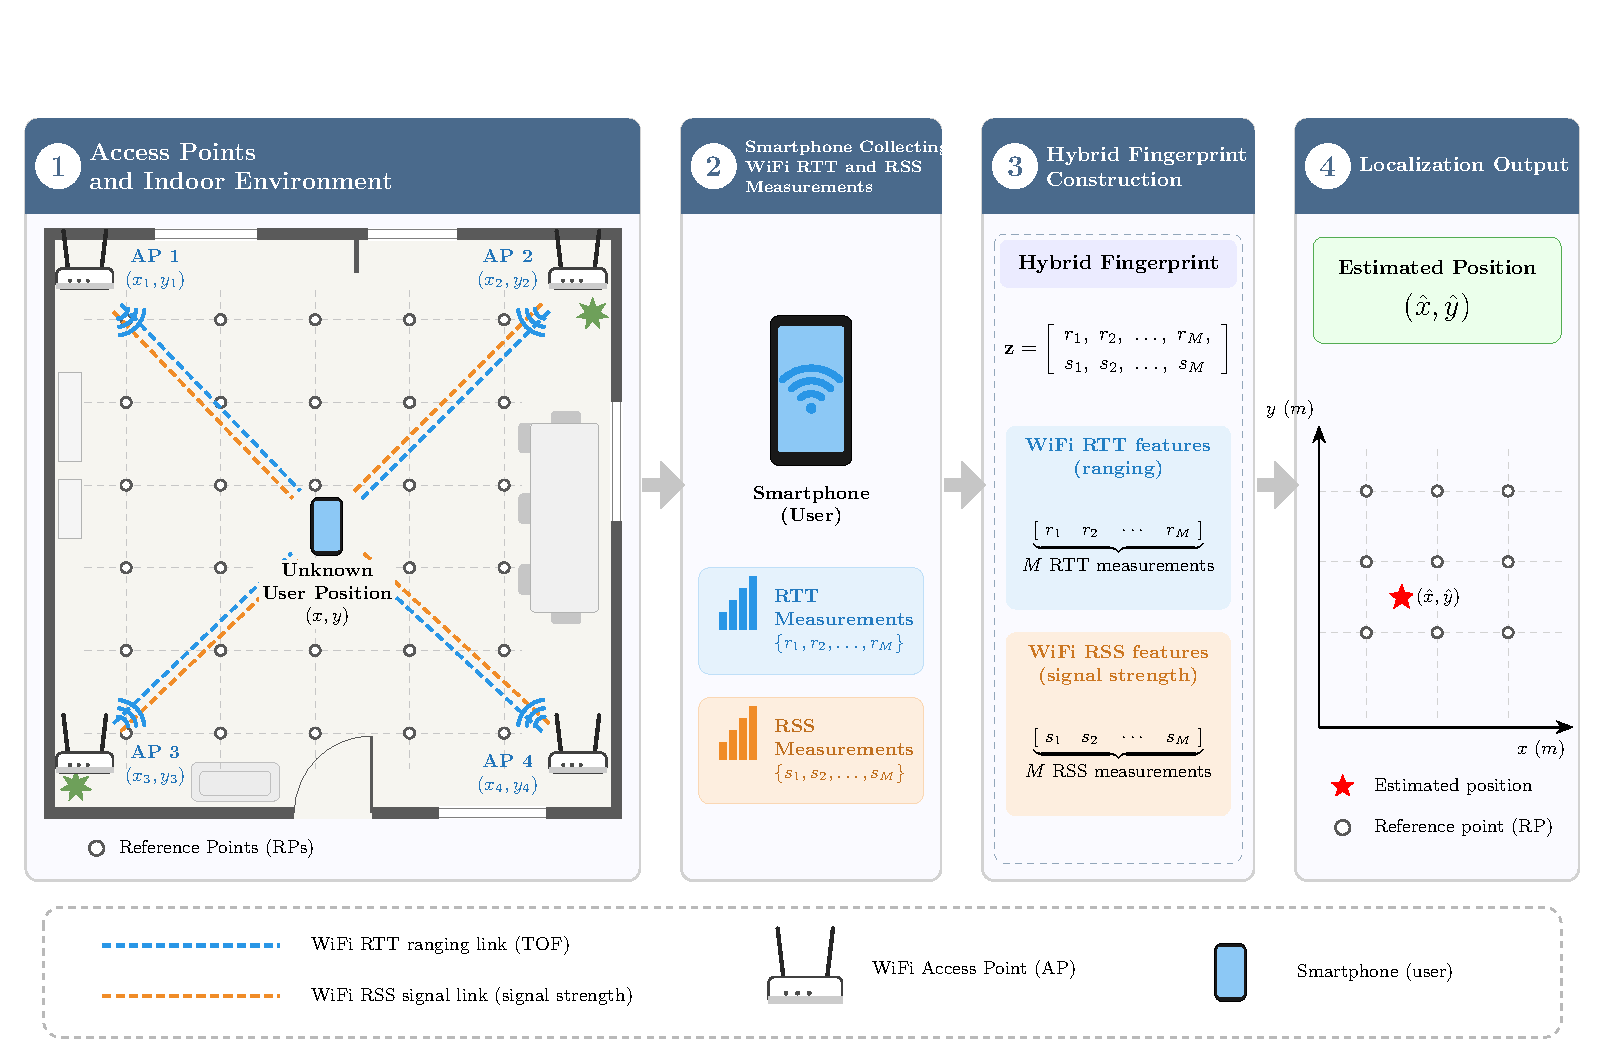
\includegraphics[width=\textwidth]{figures/methodology/fig01_system_model.pdf}
	\caption{System model of the hybrid Wi-Fi RTT--RSS indoor positioning system. A mobile device collects RTT ranging and RSS measurements from surrounding Wi-Fi access points. The measurements are concatenated into a hybrid fingerprint and mapped by the learned positioning model to an estimated two-dimensional user position.}
	\label{fig:system_model}
\end{figure*}

Rather than imposing an explicit propagation model, we follow a fingerprinting formulation. The measurements of one scan form the hybrid fingerprint
\begin{equation}
	\mathbf{z}
	=
	[r^{\mathrm{RTT}}_{1},\ldots,r^{\mathrm{RTT}}_{M},\,r^{\mathrm{RSS}}_{1},\ldots,r^{\mathrm{RSS}}_{M}]^{T}
	\in\mathbb{R}^{p},
	\label{eq:hybrid_fingerprint}
\end{equation}
with $p=2M$ features. APs that are not heard in a scan are encoded with the sentinel value of the respective dataset; no artificial distance is imputed.

\subsection{Fingerprint Database and Reference-Point Groups}

During the offline phase, scans are collected at $N_{\mathrm{RP}}$ known reference points (RPs). The database $\mathcal{D}=\{(\mathbf{z}_{i},\mathbf{u}_{i},g_i)\}_{i=1}^{N}$ contains $N\gg N_{\mathrm{RP}}$ scans with known positions $\mathbf{u}_{i}=[x_i,y_i]^{T}$ and RP identifiers
\begin{equation}
	g_i=g_j
	\quad\Longleftrightarrow\quad
	(x_i,y_i)=(x_j,y_j).
	\label{eq:rp_group}
\end{equation}
In the datasets used here, each RP contributes 100--120 scans per acquisition session. A regression function $f:\mathbb{R}^{p}\rightarrow\mathbb{R}^{2}$, $\hat{\mathbf{u}}=f(\mathbf{z})$, is learned from $\mathcal{D}$.

The grouping defines two evaluation questions. In \emph{sample-level} evaluation, scans of the same RP can appear in training and test data, so the model is asked to recognize new scans at already-surveyed locations. In \emph{RP-disjoint} evaluation, $\mathcal{G}_{\mathrm{train}}\cap\mathcal{G}_{\mathrm{test}}=\varnothing$, so the model must estimate positions at unsurveyed locations. Both are reported in this work, but never mixed.

\subsection{Localization Metrics}
\label{subsec:metrics}

For a test set of $N_t$ scans, the Euclidean error of scan $i$ is $e_i=\|\mathbf{u}_{i}-\hat{\mathbf{u}}_{i}\|_{2}$, with positions expressed in metres (for Dataset~I, grid coordinates are multiplied by the grid spacing $\Delta$ first), and the true two-dimensional RMSE is
\begin{equation}
	\mathrm{RMSE}_{2D}
	=
	\sqrt{\frac{1}{N_t}\sum_{i=1}^{N_t}e_i^{2}}.
	\label{eq:rmse2d}
\end{equation}
We also report the mean error and the $50$th, $90$th, and $95$th percentiles $P_{50}$, $P_{90}$, and $P_{95}$ of $e_i$, because an improvement of the average does not imply an improvement of the tail.

For comparison with the published hybrid RTT--RSS baseline~\cite{feng2026robust}, we additionally report the \emph{paper-compatible} metric
\begin{equation}
	E_{\mathrm{paper}}
	=
	\frac{\mathrm{RMSE}_{x}+\mathrm{RMSE}_{y}}{2}\,\Delta,
	\label{eq:paper_metric}
\end{equation}
where
\begin{align}
	\mathrm{RMSE}_{x}&=\sqrt{\frac{1}{N_t}\sum_{i=1}^{N_t}(x_i-\hat{x}_i)^{2}},\\
	\mathrm{RMSE}_{y}&=\sqrt{\frac{1}{N_t}\sum_{i=1}^{N_t}(y_i-\hat{y}_i)^{2}},
\end{align}
and $\Delta$ is the grid spacing that converts the dataset's coordinate units into metres. Because it averages per-coordinate errors, $E_{\mathrm{paper}}$ is about $\sqrt{2}$ times smaller than $\mathrm{RMSE}_{2D}$ for isotropic errors; the two are never treated as interchangeable.

\subsection{Problem Statement}

Given $\mathcal{D}$, the objective is a positioning model that (i) minimizes the localization error at unsurveyed locations, (ii) remains cheap to train and to evaluate online, (iii) is configured and validated without leakage between scans of the same RP, and (iv) optionally returns a region $\mathcal{C}_{1-\alpha}(\mathbf{z})\subset\mathbb{R}^{2}$ that contains the true position with probability at least $1-\alpha$. Section~\ref{sec:proposed_method} addresses (i)--(iii) through the subspace ratio of a Random Forest and (iv) through conformal calibration.

\section{Proposed Method}
\label{sec:proposed_method}

The framework combines a random-subspace Random Forest (RF) point predictor, RP-aware validation, final training on all RPs, and conformal uncertainty regions computed from RP-grouped residuals (Fig.~\ref{fig:overall_framework}).

\begin{figure*}[!t]
	\centering
	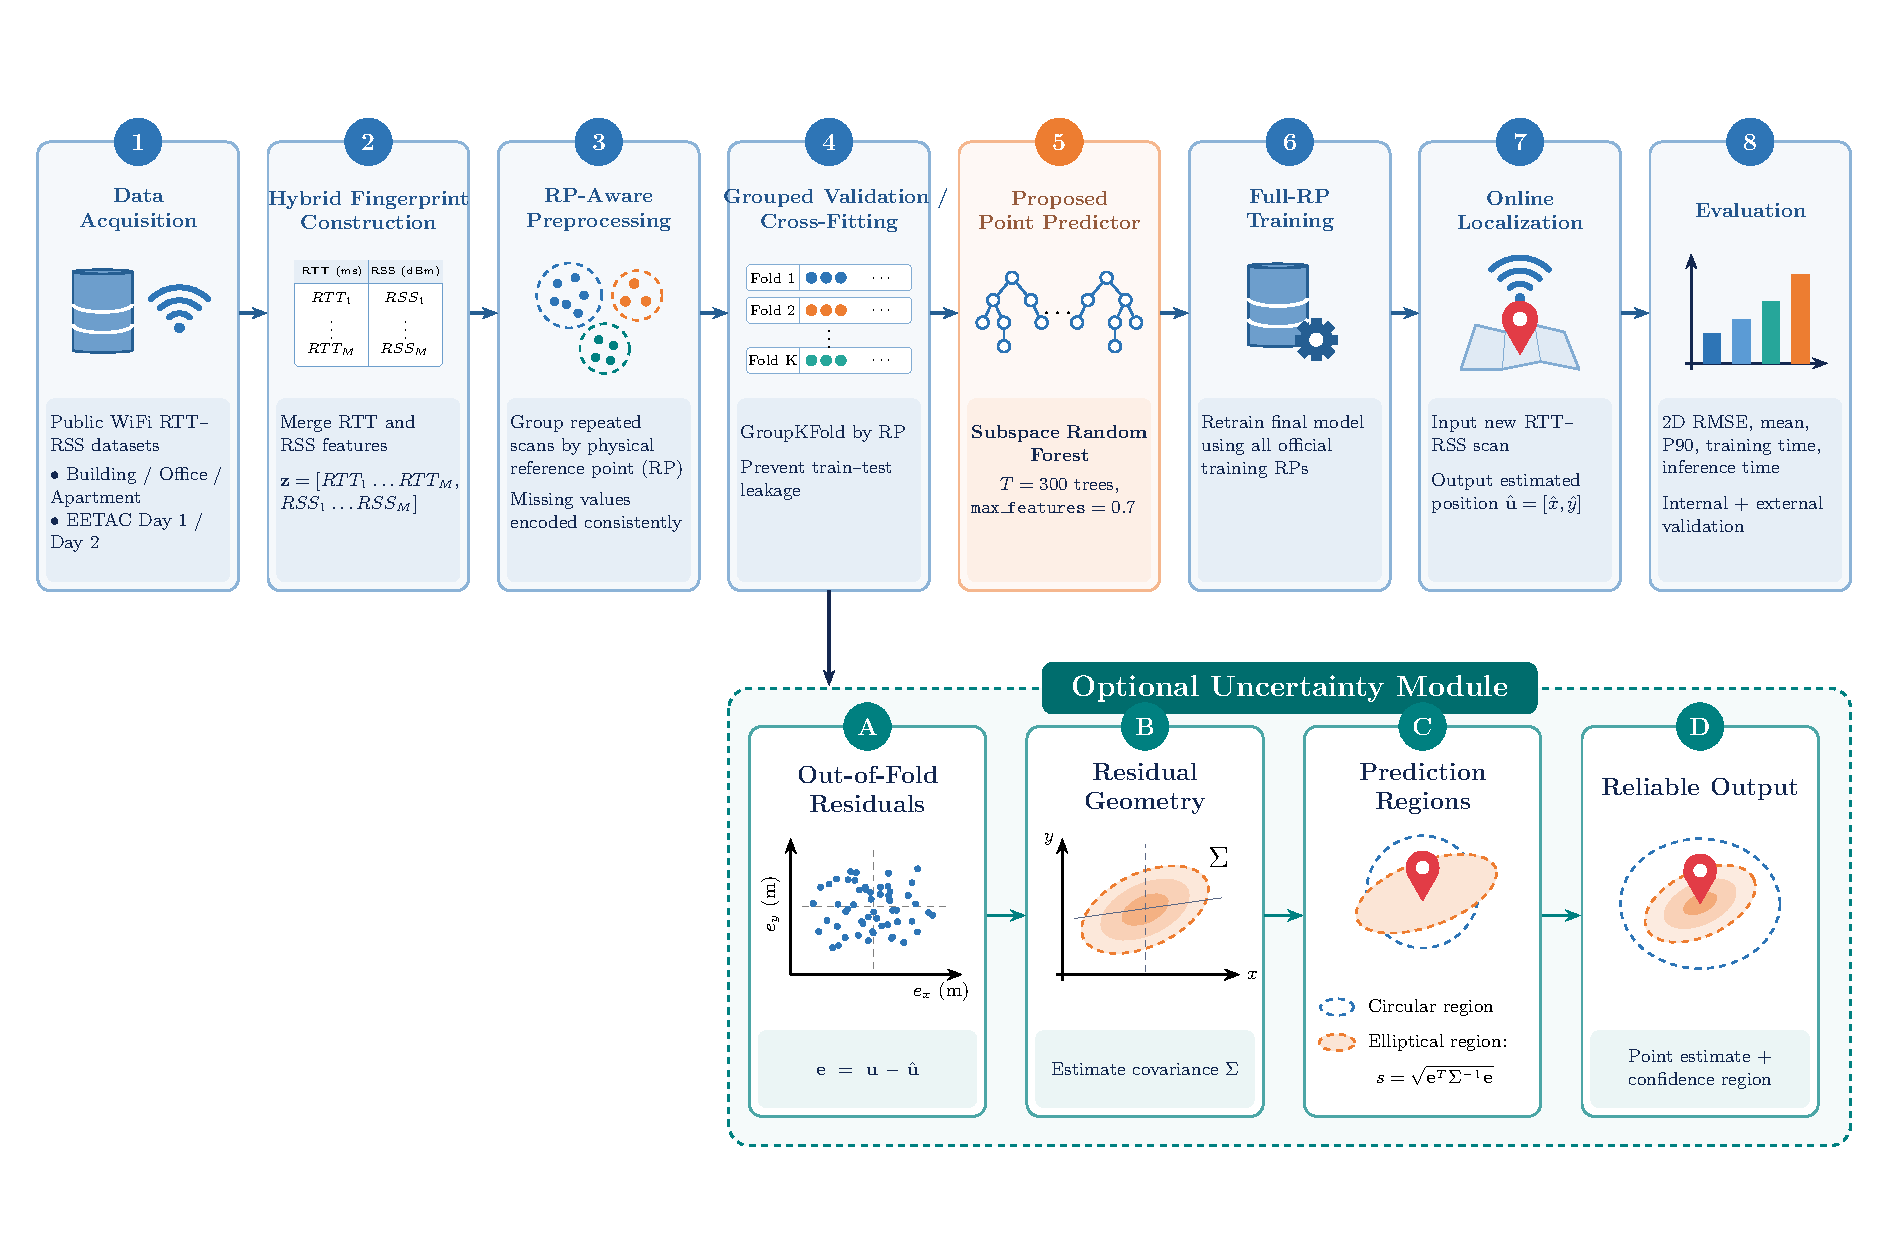
\includegraphics[width=\textwidth]{figures/methodology/fig02_framework.pdf}
	\caption{Overall workflow of the proposed hybrid Wi-Fi RTT--RSS indoor localization framework. Hybrid RTT and RSS measurements are first organized into fingerprint vectors and grouped according to their physical reference-point coordinates. A random-subspace Random Forest is used for point localization, while grouped out-of-fold residuals characterize positioning uncertainty. The final localization model is trained using all available training reference points.}
	\label{fig:overall_framework}
\end{figure*}

% ============================================================
\subsection{Random-Subspace Hybrid RTT--RSS Random Forest}
\label{subsec:subspace_rf}

An RF regressor consists of $T$ trees $h_t:\mathbb{R}^{p}\rightarrow\mathbb{R}^{2}$, each grown on a bootstrap sample of $\mathcal{D}$, and predicts
\begin{equation}
	\hat{\mathbf{u}}
	=
	f(\mathbf{z})
	=
	\frac{1}{T}\sum_{t=1}^{T}h_t(\mathbf{z}).
	\label{eq:rf_prediction}
\end{equation}
At every node, the split is chosen among a random subset of $m_{\mathrm{try}}$ of the $p$ features,
\begin{equation}
	m_{\mathrm{try}}
	=
	\max\left(1,\lfloor \rho p\rfloor\right),
	\qquad \rho\in(0,1].
	\label{eq:mtry}
\end{equation}
The full-feature configuration used in prior hybrid RTT--RSS work, $\rho=1$, is bagging of regression trees: the only source of diversity is the bootstrap sample, and the same dominant features can shape most splits of most trees. Hybrid fingerprints make this costly, because the RTT and RSS of one AP and the measurements of neighboring APs carry overlapping spatial information, while NLOS propagation and visibility changes make individual features intermittently unreliable. The proposed configuration uses $\rho=0.7$ and $T=300$ (Fig.~\ref{fig:rf_subspace}). The deployed model remains a single $T$-tree ensemble evaluated by Eq.~\eqref{eq:rf_prediction}.

\begin{figure*}[!t]
	\centering
	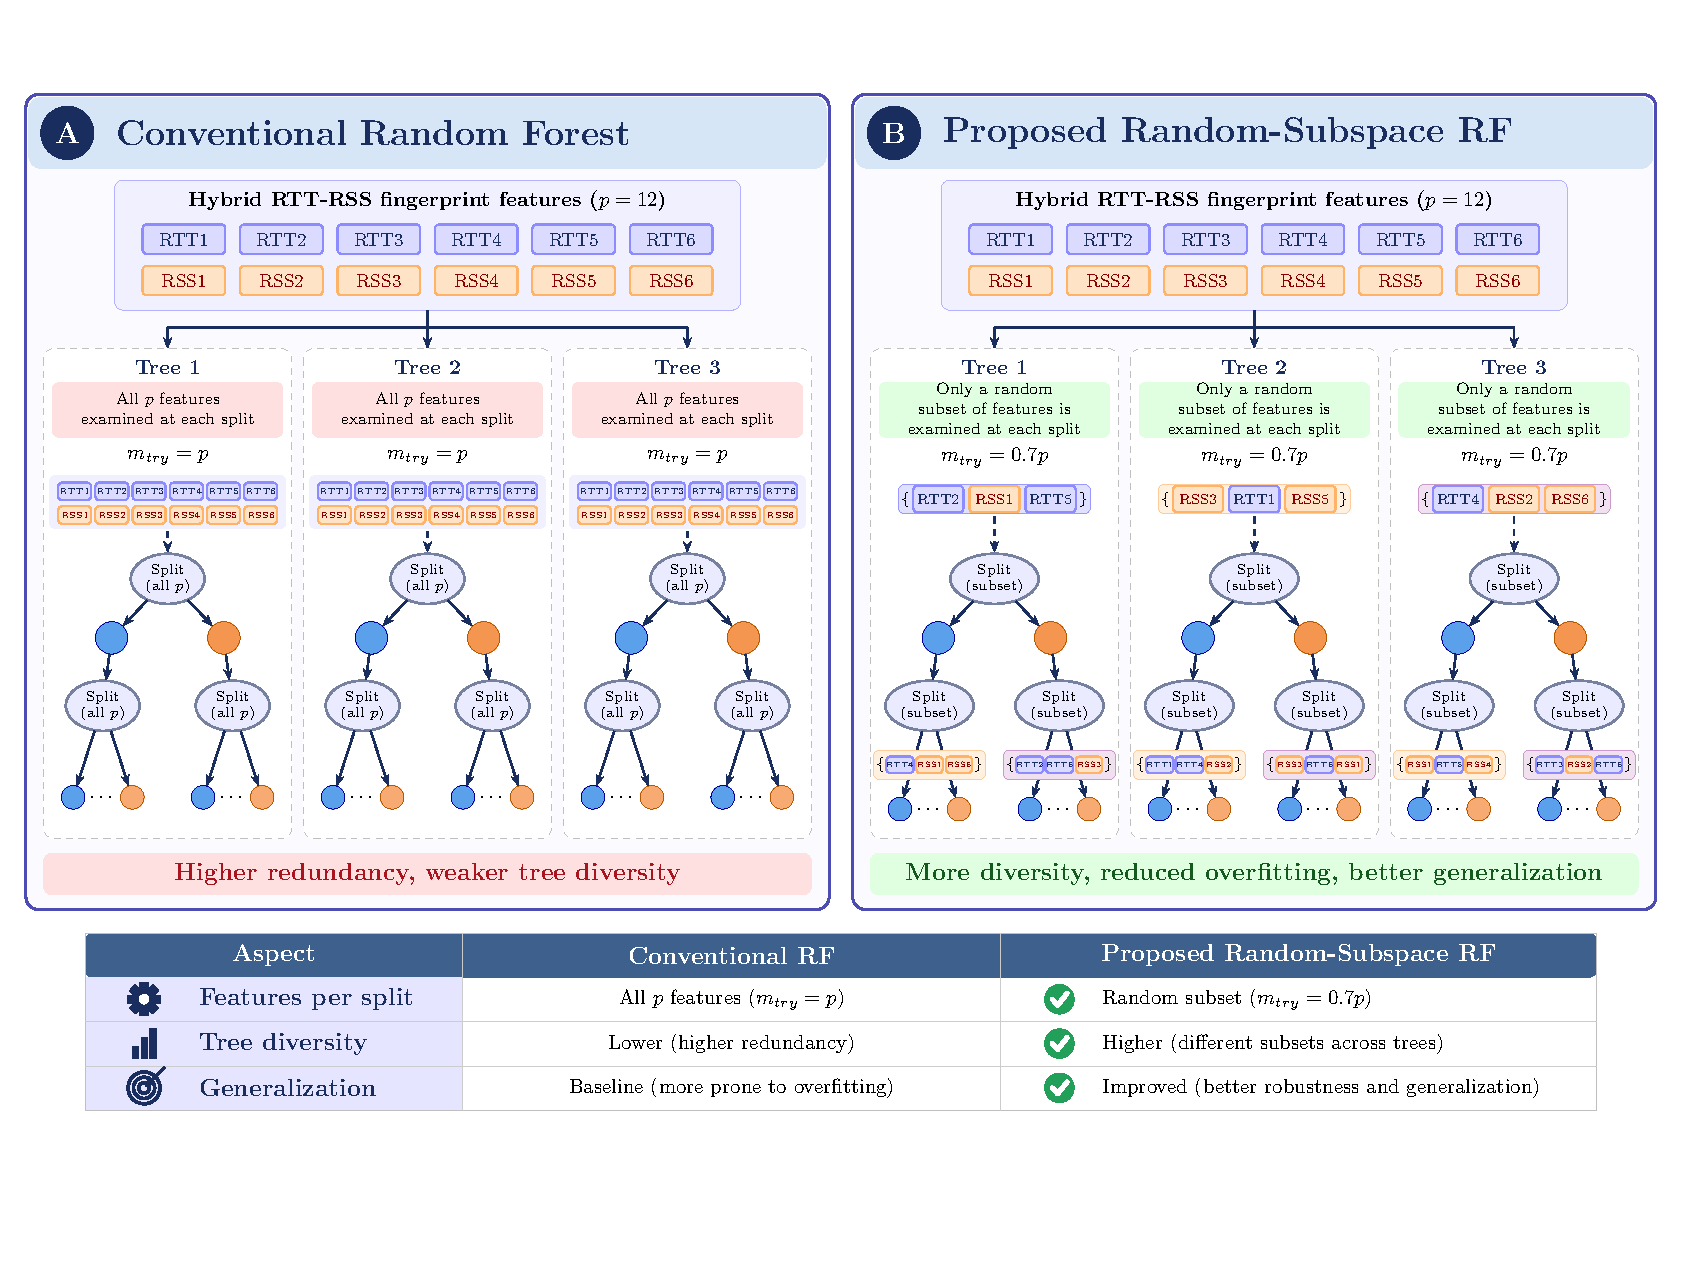
\includegraphics[width=\textwidth]{figures/methodology/fig03_rf_vs_subspace_rf.pdf}
	\caption{Conventional full-feature Random Forest and the proposed random-subspace Random Forest. In the conventional model, all $p$ hybrid RTT--RSS features are eligible at each split. The proposed model randomly exposes approximately $0.7p$ candidate features at each node, increasing ensemble diversity and reducing dependence on redundant or unstable measurements.}
	\label{fig:rf_subspace}
\end{figure*}

Per-split subsampling is a form of regularization whose optimal strength depends on the signal-to-noise ratio~\cite{mentch2020randomization}. Estimating positions between surveyed RPs is an interpolation problem that becomes noisier as the radio map becomes sparser. We therefore hypothesize that the optimal $\rho$ decreases with radio-map density; this is tested in Section~\ref{subsec:density_results}.

% ============================================================
\subsection{RP-Aware Validation}
\label{subsec:rp_grouping}

For grouped $K$-fold validation, the set of RP identifiers is partitioned into disjoint folds $\mathbb{G}^{(1)},\ldots,\mathbb{G}^{(K)}$; the model of fold $k$ is trained on all scans whose RP is not in $\mathbb{G}^{(k)}$ and predicts the scans of $\mathbb{G}^{(k)}$. Metrics are computed on the pooled out-of-fold predictions of all folds. Figure~\ref{fig:rp_validation} contrasts this protocol with sample-level splitting.

\begin{figure*}[!t]
	\centering
	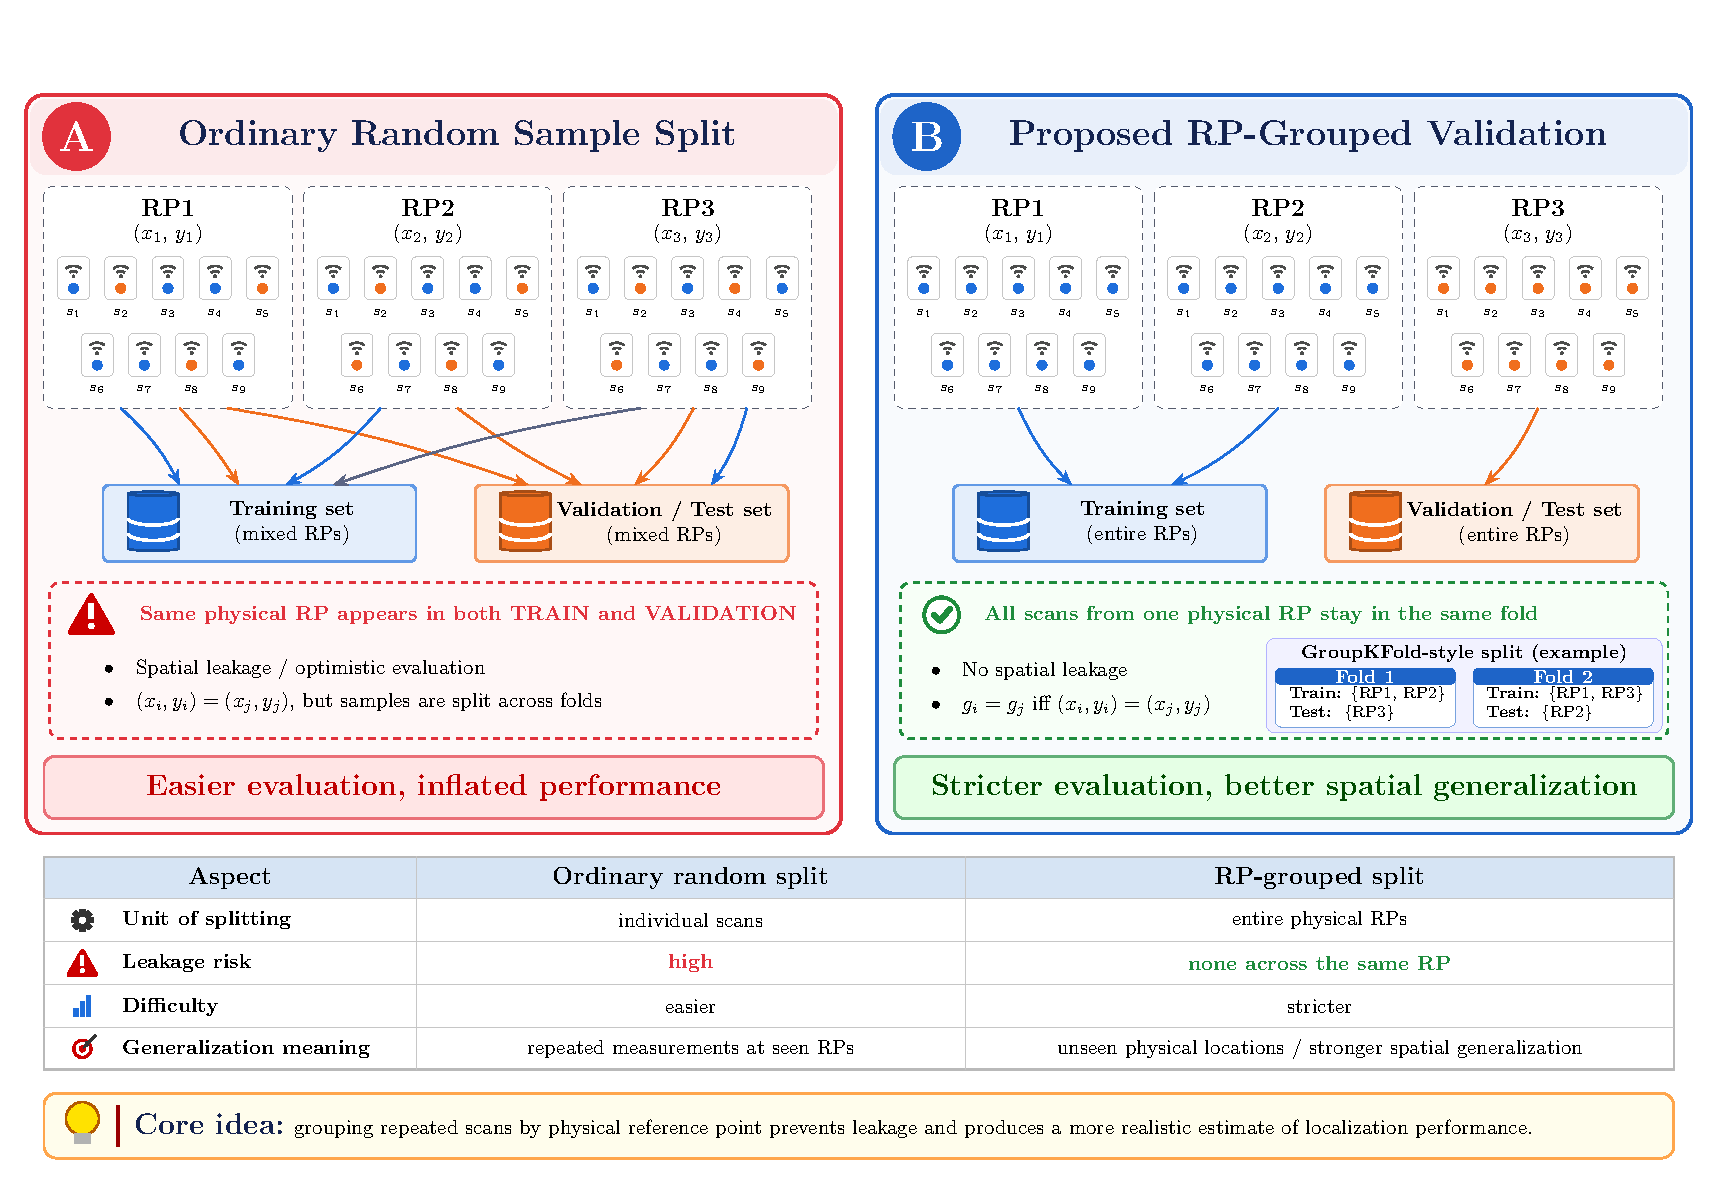
\includegraphics[width=\textwidth]{figures/methodology/fig04_rp_grouped_validation.pdf}
	\caption{Random sample-level splitting versus reference-point-aware validation. With row-level splitting, repeated scans collected at the same physical RP may appear in both training and validation subsets. RP-grouped validation keeps all measurements from one physical position in the same partition, enabling evaluation on physically unseen reference points.}
	\label{fig:rp_validation}
\end{figure*}

% ============================================================
\subsection{Choice of the Subspace Ratio}
\label{subsec:model_selection}

A natural way to select $\rho$ is to minimize a validation loss over a candidate set $\mathcal{R}$,
\begin{equation}
	\rho^{*}
	=
	\arg\min_{\rho\in\mathcal{R}}
	\mathcal{L}_{\mathrm{val}}(\rho),
	\label{eq:rho_selection}
\end{equation}
where $\mathcal{L}_{\mathrm{val}}$ is the out-of-bag (OOB) error of the forest, a sample-level $K$-fold cross-validation (CV) error, or an RP-grouped CV error. In fingerprinting, each estimator is biased in a specific way. OOB and sample-level CV evaluate each scan with trees trained on other scans of the same RP, so they measure fingerprint recognition and produce errors far below the test error. RP-grouped CV removes this leakage, but its fold models are trained on $(K-1)/K$ of the RPs, i.e., on a sparser radio map than the final model. If the optimal ratio depends on density, RP-grouped CV selects a ratio that is too small for the full-density model.

We therefore do not select $\rho$ by Eq.~\eqref{eq:rho_selection}. The proposed configuration uses the fixed default $\rho=0.7$, set during method development and frozen before external evaluation. Its quality is assessed afterwards by its regret on the official RP-disjoint test sets, with $\mathcal{L}_{\mathrm{test}}$ the paper-compatible error of Eq.~\eqref{eq:paper_metric},
\begin{equation}
	\mathrm{Regret}(\rho)
	=
	\frac{\mathcal{L}_{\mathrm{test}}(\rho)}{\min_{\rho'\in\mathcal{R}}\mathcal{L}_{\mathrm{test}}(\rho')}-1,
	\label{eq:regret}
\end{equation}
and compared with the regret of the data-driven rules above, of a leave-one-environment-out rule that picks the ratio minimizing the worst RP-grouped CV regret on the other environments, and of the defaults $\rho=1$ and $m_{\mathrm{try}}=\lfloor p/3\rfloor$~\cite{breiman2001random}. The test sets score these rules but never choose $\rho$.

After validation, the final model $f^{*}$ is trained on all available training RPs (Algorithm~\ref{alg:subspace_rf}), since every withheld RP makes the radio map sparser.

\begin{algorithm}[t]
	\caption{RP-Aware Random-Subspace RTT--RSS Localization}
	\label{alg:subspace_rf}
	\begin{algorithmic}[1]

		\Require
		Fingerprint dataset
		$\mathcal{D}=\{(\mathbf{z}_i,\mathbf{u}_i,g_i)\}_{i=1}^{N}$;
		number of trees $T$;
		fixed subspace ratio $\rho$ (default $0.7$);
		number of grouped folds $K$

		\Ensure
		Final positioning model $f^{*}$; RP-disjoint validation estimate

		\State $m_{\mathrm{try}} \leftarrow \max(1,\lfloor \rho p \rfloor)$

		\For{$k=1$ to $K$}
		\Comment{validation only}

		\State Construct RP-disjoint training and validation sets:
		$\mathcal{G}^{(k)}_{\mathrm{train}}\cap\mathcal{G}^{(k)}_{\mathrm{val}}=\varnothing$

		\State $f^{(k)} \leftarrow \mathrm{RF}\left(\mathcal{D}^{(-k)};\,T,\,m_{\mathrm{try}}\right)$

		\State $\hat{\mathbf{u}}_i^{\mathrm{OOF}} \leftarrow f^{(k)}(\mathbf{z}_i)$ for all $i$ with $g_i\in\mathcal{G}^{(k)}_{\mathrm{val}}$

		\EndFor

		\State Report metrics on the pooled out-of-fold predictions
		$\{\hat{\mathbf{u}}_i^{\mathrm{OOF}}\}_{i=1}^{N}$

		\State Train the final model on all available training RPs:
		\[
		f^{*}
		\leftarrow
		\mathrm{RF}
		\left(
		\mathcal{D};\,
		T,\,
		m_{\mathrm{try}}
		\right)
		\]

		\State \Return $f^{*}$

	\end{algorithmic}
\end{algorithm}


% ============================================================
\subsection{Grouped Out-of-Fold Residuals}
\label{subsec:oof_residual}

Uncertainty estimation requires residuals of predictions at locations the model has not seen. For each scan $i$, the RP-grouped out-of-fold prediction $\hat{\mathbf{u}}_{i}^{\mathrm{OOF}}$ is produced by the fold model that excluded the RP of $i$, and the residual is
\begin{equation}
	\boldsymbol{\epsilon}_{i}
	=
	\mathbf{u}_{i}-\hat{\mathbf{u}}_{i}^{\mathrm{OOF}}
	=
	\left[x_i-\hat{x}_i^{\mathrm{OOF}},\;y_i-\hat{y}_i^{\mathrm{OOF}}\right]^{T}.
	\label{eq:oof_residual}
\end{equation}

% ============================================================
\subsection{Circular and Covariance-Aware Elliptical Regions}
\label{subsec:circle_uncertainty}

The isotropic nonconformity score is $s_i^{\mathrm{circ}}=\|\boldsymbol{\epsilon}_{i}\|_{2}$, which yields the circular region
\begin{equation}
	\mathcal{C}_{\mathrm{circ}}
	=
	\left\{\mathbf{u}:\|\mathbf{u}-\hat{\mathbf{u}}^{*}\|_{2}\leq q_{\mathrm{circ}}\right\},
	\qquad
	A_{\mathrm{circ}}=\pi q_{\mathrm{circ}}^{2},
	\label{eq:circle_region}
\end{equation}
around a new prediction $\hat{\mathbf{u}}^{*}$, where $q_{\mathrm{circ}}$ is a calibrated quantile of the scores (Section~\ref{subsec:strict_conformal}).

Indoor errors are often anisotropic because of corridors, walls, and AP geometry. With the regularized residual covariance $\boldsymbol{\Sigma}=\mathrm{Cov}(\{\boldsymbol{\epsilon}_{i}\})+\lambda\mathbf{I}$, where $\lambda$ is a small ridge for numerical stability, the Mahalanobis score
\begin{equation}
	s_{i}^{\mathrm{ell}}
	=
	\sqrt{\boldsymbol{\epsilon}_{i}^{T}\boldsymbol{\Sigma}^{-1}\boldsymbol{\epsilon}_{i}}
	\label{eq:mahalanobis_score}
\end{equation}
yields the elliptical region (Fig.~\ref{fig:circle_ellipse})
\begin{align}
	\mathcal{C}_{\mathrm{ell}}
	&=
	\left\{\mathbf{u}:(\mathbf{u}-\hat{\mathbf{u}}^{*})^{T}\boldsymbol{\Sigma}^{-1}(\mathbf{u}-\hat{\mathbf{u}}^{*})\leq q_{\mathrm{ell}}^{2}\right\},
	\label{eq:ellipse_region}\\
	A_{\mathrm{ell}}
	&=
	\pi q_{\mathrm{ell}}^{2}\sqrt{\det\boldsymbol{\Sigma}}.
	\label{eq:ellipse_area}
\end{align}
A region is evaluated by its area together with its empirical coverage on the test set,
\begin{equation}
	\mathrm{Coverage}
	=
	\frac{1}{N_t}\sum_{i=1}^{N_t}\mathbb{I}\left[\mathbf{u}_{i}\in\mathcal{C}_{i}\right],
	\label{eq:coverage}
\end{equation}
and a smaller region is only better at equal coverage.

\begin{figure}[!t]
	\centering
	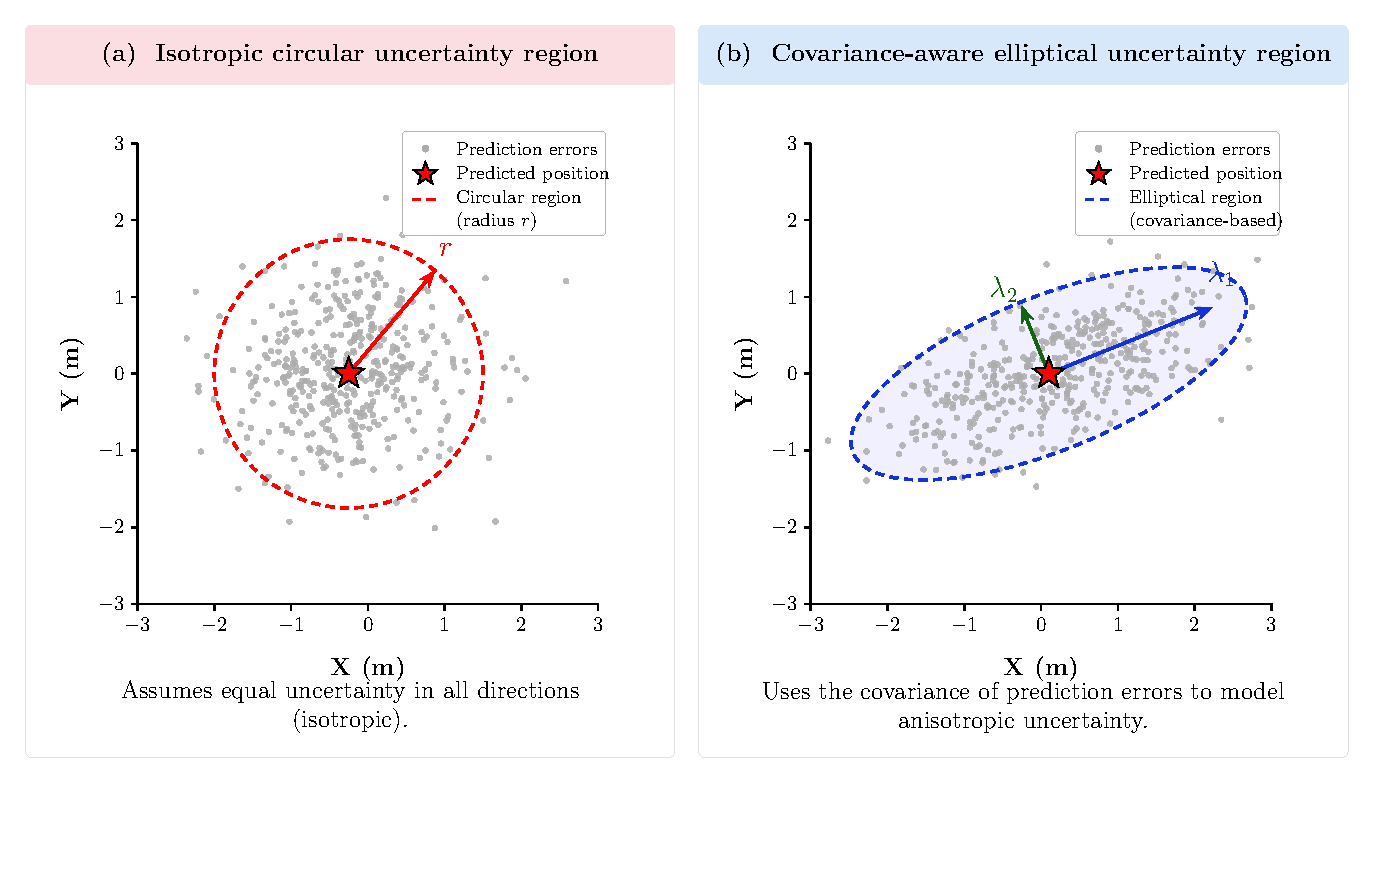
\includegraphics[width=\columnwidth]{figures/methodology/fig05_circle_vs_ellipse.pdf}
	\caption{Circular and covariance-aware elliptical uncertainty regions. The circular construction assigns the same uncertainty scale in every direction. The covariance-aware ellipse adapts its orientation and axis lengths according to the spatial covariance of localization residuals.}
	\label{fig:circle_ellipse}
\end{figure}

% ============================================================
\subsection{Calibration}
\label{subsec:strict_conformal}

\subsubsection{Scan-Level Split Conformal}
The training RPs are split into disjoint fitting and calibration sets, $\mathbb{G}_{\mathrm{fit}}\cap\mathbb{G}_{\mathrm{cal}}=\varnothing$. The point predictor is trained on $\mathcal{D}_{\mathrm{fit}}$, $\boldsymbol{\Sigma}$ is estimated from grouped OOF residuals inside $\mathcal{D}_{\mathrm{fit}}$, and the threshold, $q_{\mathrm{circ}}$ or $q_{\mathrm{ell}}$ depending on the score, is computed from the sorted scores $s_{(1)}\leq\cdots\leq s_{(n)}$ of the calibration scans,
\begin{equation}
	q_{\alpha}
	=
	s_{\left(\left\lceil(n+1)(1-\alpha)\right\rceil\right)},
	\label{eq:conformal_quantile}
\end{equation}
with $n=n_{\mathrm{cal}}$, the number of calibration scans. This is standard practice in conformal indoor positioning~\cite{feng2026robust}, and it gives the marginal coverage guarantee $P(\mathbf{u}\in\mathcal{C})\geq1-\alpha$ when calibration and test scans are exchangeable~\cite{lei2018distribution}.

\subsubsection{Group Split Conformal}
\label{subsubsec:group_conformal}
In fingerprinting, the calibration scans are not exchangeable with the test scans: they come from $G$ held-out RPs with $\sim$120 nearly identical scans each, whereas the test scans come from other RPs. The exchangeable units are the RPs, so the effective calibration sample size is $G$, not $n_{\mathrm{cal}}$. Following Dunn et al.~\cite{Dunn02102023}, we draw one scan at random from each calibration RP and apply Eq.~\eqref{eq:conformal_quantile} to these $G$ scores, i.e., with $n=G$. If the RPs are exchangeable, the score of one random scan of a new test RP is exchangeable with these $G$ scores, and the resulting region has the marginal coverage guarantee for a scan of a new RP. The guarantee holds on average over the calibration draw; individual calibration sets can cover more or less. The construction requires $\lceil(G+1)(1-\alpha)\rceil\leq G$, i.e., $G\geq1/\alpha-1$: at least 9 calibration RPs for $90\%$ and 19 for $95\%$. With fewer RPs, no finite distribution-free region exists.

\subsubsection{RP-Count Conservative Correction}
\label{subsubsec:rp_corrected}
As a simple alternative that uses all calibration scans, we also evaluate an RP-count-based correction that pools the scores but computes the finite-sample level from $G$:
\begin{align}
	q_{\alpha}^{\mathrm{RP}}
	&=
	Q_{\ell_G}\!\left(\{s_1,\ldots,s_{n_{\mathrm{cal}}}\}\right),
	\label{eq:rp_corrected_quantile}\\
	\ell_G
	&=
	\min\!\left(1,\frac{\lceil (G+1)(1-\alpha)\rceil}{G}\right),
	\label{eq:rp_level}
\end{align}
where $Q_{\ell}$ is the empirical $\ell$-quantile (``higher'' interpolation). Because $\ell_G$ is never smaller than the scan-level level, $q_{\alpha}^{\mathrm{RP}}\geq q_{\alpha}$. This correction is a conservative heuristic without a finite-sample guarantee, and it is evaluated empirically. When $G<2/\alpha-1$ (fewer than 19 calibration RPs at $90\%$ or 39 at $95\%$), $\ell_G=1$ and the threshold becomes the largest calibration score.

\subsubsection{Full-Training Grouped-OOF Variant}
\label{subsec:empirical_oof}
Reserving calibration RPs costs point accuracy. In this variant, the final predictor is trained on all training RPs, and $\boldsymbol{\Sigma}$ and the thresholds are computed from the grouped OOF residuals of Section~\ref{subsec:oof_residual}. Because these residuals come from several fold models rather than from one predictor and an independent calibration set, the variant is an empirical estimator without the split-conformal guarantee; cross-fitted constructions such as CV+ would be required for one~\cite{barber2021jackknife}. The procedure is summarized in Algorithm~\ref{alg:uncertainty}.

\begin{algorithm}[t]
	\caption{RP-Grouped Covariance-Aware Uncertainty Estimation}
	\label{alg:uncertainty}
	\begin{algorithmic}[1]
		
		\Require
		Training dataset
		$\mathcal{D}=\{(\mathbf{z}_i,\mathbf{u}_i,g_i)\}_{i=1}^{N}$;
		number of folds $K$;
		confidence level $1-\alpha$;
		fixed RF parameters $T=300$ and $\rho=0.7$
		
		\Ensure
		Residual covariance $\boldsymbol{\Sigma}$;
		circular threshold $q_{\mathrm{circ}}$;
		elliptical threshold $q_{\mathrm{ell}}$
		
		\State Partition physical RPs into $K$ disjoint groups
		
		\For{$k=1$ to $K$}
		
		\State Train the fold model without RP group $k$:
		\[
		f^{(-k)}
		\leftarrow
		\mathrm{RF}
		\left(
		\mathcal{D}^{(-k)};
		300,
		0.7
		\right)
		\]
		
		\For{each sample $i$ in held-out RP fold $k$}
		
		\State Compute out-of-fold prediction:
		\[
		\hat{\mathbf{u}}_i^{\mathrm{OOF}}
		=
		f^{(-k)}(\mathbf{z}_i)
		\]
		
		\State Compute residual:
		\[
		\boldsymbol{\epsilon}_i
		=
		\mathbf{u}_i
		-
		\hat{\mathbf{u}}_i^{\mathrm{OOF}}
		\]
		
		\EndFor
		
		\EndFor
		
		\State Estimate residual covariance:
		\[
		\boldsymbol{\Sigma}
		=
		\mathrm{Cov}
		\left(
		\{\boldsymbol{\epsilon}_i\}
		\right)
		+
		\lambda\mathbf{I}
		\]
		
		\For{each residual $\boldsymbol{\epsilon}_i$}
		
		\State Circular score:
		\[
		s_i^{\mathrm{circ}}
		=
		\|\boldsymbol{\epsilon}_i\|_2
		\]
		
		\State Elliptical score:
		\[
		s_i^{\mathrm{ell}}
		=
		\sqrt{
			\boldsymbol{\epsilon}_i^{T}
			\boldsymbol{\Sigma}^{-1}
			\boldsymbol{\epsilon}_i
		}
		\]
		
		\EndFor
		
		\State Compute uncertainty thresholds with the finite-sample level of Eq.~\eqref{eq:conformal_quantile}, $n=N$:
		\[
		q_{\mathrm{circ}}
		=
		s^{\mathrm{circ}}_{\left(\lceil (N+1)(1-\alpha)\rceil\right)},
		\qquad
		q_{\mathrm{ell}}
		=
		s^{\mathrm{ell}}_{\left(\lceil (N+1)(1-\alpha)\rceil\right)}
		\]
		
		\State \Return
		$\boldsymbol{\Sigma}$,
		$q_{\mathrm{circ}}$,
		$q_{\mathrm{ell}}$
		
	\end{algorithmic}
\end{algorithm}

% ============================================================
\subsection{Computational Complexity}
\label{subsec:complexity}

Training an RF costs approximately $\mathcal{O}(T N m_{\mathrm{try}}\log N)$ for $N$ training scans, so $\rho=0.7$ reduces the number of candidate-feature evaluations per split by $30\%$; measured wall-clock times also depend on tree depth, parallelization, and implementation and are therefore reported explicitly. Inference traverses one root-to-leaf path per tree, $\mathcal{O}(T D_t)$ for average depth $D_t$, so model size and latency are controlled mainly by $T$ and the leaf size. Grouped fold models are needed only offline. Online, the system evaluates $f^{*}$ and, if requested, returns $\mathcal{C}_{1-\alpha}$, which adds only a two-dimensional quadratic form.

\section{Experimental Setup}
\label{sec:experimental_setup}

The experiments address six questions: (1) whether the published full-feature hybrid RF can be reproduced; (2) whether $\rho=0.7$ improves on it under otherwise identical settings; (3) whether the improvement holds on an independent dataset and across acquisition days without retuning; (4) how the optimal ratio depends on radio-map density and how it can be chosen; (5) how the configuration compares with literature ensembles and how small the model can be made; and (6) whether conformal regions keep their coverage when calibration scans are clustered by RP. The protocols were fixed before the final tables and figures were generated.

% ============================================================
\subsection{Dataset I: Hybrid RTT--RSS Benchmark}
\label{subsec:dataset_original}

The first dataset is the public hybrid Wi-Fi RTT--RSS benchmark of Feng et al.~\cite{feng2026robust}, collected with an LG G8X ThinQ smartphone in a university building floor with mixed LOS/NLOS conditions, a LOS-dominated office, and an apartment with one AP in NLOS for most RPs (Table~\ref{tab:dataset_summary}). Missing measurements are encoded with the dataset's sentinels, $100000$~mm for RTT and $-200$~dBm for RSS; no imputation, normalization, or feature transformation is applied. Coordinates are given in grid units and converted to metres with the grid spacing $\Delta$ of each environment.

\begin{table}[!t]
	\centering
	\caption{Hybrid RTT--RSS benchmark datasets. Sample counts correspond to the distributed files used in this study.}
	\label{tab:dataset_summary}
	\footnotesize
	\setlength{\tabcolsep}{3.5pt}
	\begin{tabular}{lccc}
		\toprule
		 & Building & Office & Apartment \\
		\midrule
		Area (m$^2$) & $92\times15$ & $5.5\times4.5$ & $7.7\times9.4$ \\
		Grid spacing $\Delta$ (m) & 0.60 & 0.455 & 0.48 \\
		APs ($p=2M$ features) & 13 (26) & 3 (6) & 4 (8) \\
		Training / test RPs & 483 / 159 & 28 / 9 & 81 / 29 \\
		Scans per RP & 120 & 120 & 120 \\
		Training / test scans & 57,960 / 19,080 & 3,360 / 1,080 & 9,720 / 3,480 \\
		\bottomrule
	\end{tabular}
\end{table}

The official training and test files are RP-disjoint in all three environments: no test coordinate occurs in the training file. The official test therefore measures generalization to unseen locations at the full training density, and it is never used to choose $\rho$. The distributed Office files contain 3,360 training and 1,080 test scans, slightly different from the 3,240 and 1,200 stated in~\cite{feng2026robust}; all results use the distributed files.

% ============================================================
\subsection{Dataset II: EETAC Auditorium}
\label{subsec:eetac_dataset}

The EETAC dataset~\cite{martinescalona2023ftm}, also used in~\cite{gonzalezdiaz2026scalable}, was collected with a Google Pixel 3a in a $19.2\times8$~m$^2$ auditorium on a $5\times5$ RP grid (spacing 4.8~m by 2~m), with about 100 scans per RP on each of two acquisition days (2,500 scans per day). RTT and RSS files are aligned scan by scan through their metadata. The raw files expose several BSSIDs per physical AP; they are grouped into physical APs, with the RSS feature defined as the strongest and the RTT feature as the median of the available BSSID values. The missing-value code $-100$ is preserved. Two configurations are used: \emph{Medium}, four Google APs, and \emph{High}, the four Google APs plus the three Linksys/Belkin APs present on both days. The two-AP configuration of~\cite{gonzalezdiaz2026scalable} is not used, because the public files do not identify which Google APs form its opposite-corner pair.

\subsection{EETAC Preprocessing and Frame Alignment}
\label{subsec:preprocessing}

The upper grid row is recorded as $y=8.1$~m on Day~1 and $y=8.0$~m on Day~2; coordinates within $0.25$~m of the canonical grid $x\in\{0,4.8,9.6,14.4,19.2\}$, $y\in\{0,2,4,6,8\}$ are snapped to it.

More importantly, the two days are not recorded in the same coordinate frame. For each RP, we compared the median RTT fingerprint of the four Google APs on Day~1 with all Day~2 RP fingerprints. Under the identity mapping, the nearest Day~2 fingerprint lies at the same coordinates for only 4 of the 25 RPs, all in the central row $y=4$~m, which is invariant under a vertical mirror. Under $y\mapsto 8-y$, it lies at the mirrored coordinates for 22 of 25 RPs; the remaining three are near-ties with a neighboring row. Day~2 is therefore expressed in a frame mirrored about $y=4$~m. Without alignment, every pooled or cross-day experiment assigns one coordinate label to two physical locations. The pipeline detects the mapping from the data, applies $y\mapsto8-y$ to Day~2 before pooling, and writes the evidence to an audit file. Accuracy does not depend on which day's frame is used as reference.

% ============================================================
\subsection{Compared Models}
\label{subsec:compared_models}

The main comparison isolates the subspace ratio: RF300-F1.0 ($\rho=1$, the full-feature baseline) and RF300-F0.7 ($\rho=0.7$) share all other settings (Table~\ref{tab:rf_configuration}). The literature baselines are described in Section~\ref{subsec:extension_protocols}.

\begin{table}[!t]
	\centering
	\caption{Random Forest configurations of the main comparison.}
	\label{tab:rf_configuration}
	\footnotesize
	\begin{tabular}{lcc}
		\toprule
		Parameter & RF300-F1.0 & RF300-F0.7 \\
		\midrule
		Number of trees $T$ & 300 & 300 \\
		Feature ratio $\rho$ & 1.0 & 0.7 \\
		Maximum depth / min. leaf size & none / 1 & none / 1 \\
		Bootstrap sampling & yes & yes \\
		\bottomrule
	\end{tabular}
\end{table}

% ============================================================
\subsection{Evaluation Protocols}
\label{subsec:evaluation_protocols}

\begin{itemize}
	\item \textbf{Official test (Dataset I).} Both models are trained on the full official training file and evaluated on the official RP-disjoint test file; the published values $0.60$, $0.38$, and $0.59$~m~\cite{feng2026robust} are used only as reference.
	\item \textbf{RP-grouped CV (Dataset I).} Five-fold \texttt{GroupKFold} on the training file with groups $g_i=(x_i,y_i)$; both models use identical folds.
	\item \textbf{EETAC sample-level CV.} Five-fold CV on the pooled, frame-aligned days, stratified by RP so that every fold contains every RP; this measures recognition of surveyed locations.
	\item \textbf{EETAC RP-grouped CV.} Five-fold CV holding out complete RPs of the $5\times5$ grid.
	\item \textbf{Cross-day.} Training on all scans of one day and testing on all scans of the other, in both directions, without any target-day data.
	\item \textbf{Training-data utilization.} RF300-F0.7 trained on the $75\%$ fitting subset of the calibration split versus all training RPs.
	\item \textbf{Uncertainty.} On Dataset I, $25\%$ of the training RPs are reserved for calibration; circles and ellipses are calibrated with the scan-level and RP-count levels and with the full-training grouped-OOF variant, at $1-\alpha\in\{0.90,0.95\}$. The test set is used only after the regions have been fixed.
\end{itemize}

\textbf{Metrics and statistics.} Localization is reported with the metrics of Section~\ref{subsec:metrics}; the paper-compatible metric is used only for comparison with~\cite{feng2026robust}. Regions are reported by empirical coverage and area. Because scans of one RP are correlated, the official-test difference between the two models is assessed with a paired cluster bootstrap that resamples complete test RPs (1000 replicates). Computational cost is reported as training time, median prediction time over five repetitions, inference time per scan, and serialized (pickle) model size.

% ============================================================
\subsection{Extension Protocols}
\label{subsec:extension_protocols}

Six additional analyses use the same data, preprocessing, and implementation, including $m_{\mathrm{try}}=\max(1,\lfloor\rho p\rfloor)$. All metrics come from the official RP-disjoint tests or from five-fold RP-grouped CV with pooled out-of-fold predictions. The extension analyses use seeds 0--9 or 0--2 as stated below, whereas the main tables use seed 42; values of the same configuration can therefore differ slightly between the main and extension tables.

\begin{enumerate}
	\item \textbf{Robustness over seeds.} The comparison $\rho=0.7$ versus $\rho=1$ is repeated with ten seeds (0--9) on the official tests and on all eight EETAC comparisons; for EETAC, a paired RP-clustered bootstrap (1000 replicates) gives 95\% intervals of the 2D RMSE difference.
	\item \textbf{Radio-map density.} The training map is thinned to $100\%$, $75\%$, $50\%$, and $25\%$ of its RPs by sampling complete RPs, and $\rho\in\{0.2,0.35,0.5,0.7,0.85,1.0\}$ is evaluated on the full official test set for Random Forests and extremely randomized trees, with the same ten random RP subsets for both.
	\item \textbf{Ratio-selection rules.} For the same grid of $\rho$, the OOB error, five-fold sample-level CV error, and five-fold RP-grouped CV error on the training file are recorded together with the official test error (seed 0); the rules of Section~\ref{subsec:model_selection} are scored by their test regret.
	\item \textbf{Literature baselines.} RF with $m_{\mathrm{try}}=\lfloor p/3\rfloor$~\cite{breiman2001random}, extremely randomized trees with all features~\cite{geurts2006extremely}, Rotation Forest~\cite{rodriguez2006rotation} (standardized features, disjoint random subsets of three features, PCA on a $75\%$ subsample per subset, 300 trees), gradient-boosted trees (500 iterations, learning rate 0.05), and distance-weighted KNN ($k=5$, standardized features), with three seeds for Office and Apartment and one seed for Building.
	\item \textbf{Calibration with clustered scans.} The split-conformal circle of RF300-F0.7 is recomputed over 20 (Building: 10) random RP-level fit/calibration splits, comparing the scan-level, group, and RP-count rules of Section~\ref{subsec:strict_conformal} on the same splits and models.
	\item \textbf{Compact forests.} $T\in\{50,100,300\}$, minimum leaf size $\{1,5,20\}$, maximum depth $\{\text{none},16\}$, and $\rho\in\{0.5,0.7,1.0\}$, trained on the full training file; serialized size and single-thread inference time are measured.
\end{enumerate}

An EETAC ratio sweep repeats the sample-level, RP-grouped, and cross-day protocols for the same grid with three seeds. Additional screening experiments are reported in the supplementary material.

\subsection{Implementation Details}
\label{subsec:implementation_details}

All experiments were implemented in Python 3.14 with scikit-learn 1.9.1, NumPy 2.4.4, SciPy 1.17.1, and joblib 1.6.0. Random Forests use \texttt{RandomForest}\allowbreak\texttt{Regressor}. The random seed is $42$ in the main pipeline and $0$--$9$ or $0$--$2$ in the extension analyses. Training uses all 20 threads of an Intel Core i5-13500HX laptop CPU with 16~GB of RAM; no GPU is used. A single orchestration script reproduces all tables and figures of the main comparison from the public data, and separate scripts reproduce the extension analyses and the EETAC frame audit.

\section{Results}
\label{sec:results}

This section first compares the proposed RF300-F0.7 configuration with the full-feature RF300-F1.0 baseline on the original benchmark and on the independent EETAC dataset. It then analyzes the subspace ratio itself (density dependence and selection), compares the configuration with literature ensembles, and reports computational cost and uncertainty calibration.

% ============================================================
\subsection{Original Benchmark Localization Accuracy}
\label{subsec:original_results}

Table~\ref{tab:original_accuracy} reports the localization results on the official Building, Office, and Apartment test sets, which are RP-disjoint from the training sets.

\begin{table*}[!t]
\centering
\caption{Point-localization performance on the original hybrid RTT--RSS benchmark (official RP-disjoint test sets). The paper-compatible metric is defined in Eq.~\eqref{eq:paper_metric}. 95\% CI: paired cluster bootstrap over test RPs (1000 replicates) of the F0.7$-$F1.0 difference in the paper-compatible metric; an interval excluding zero indicates a reliable improvement.}
\label{tab:original_accuracy}
\footnotesize
\setlength{\tabcolsep}{4pt}
\begin{tabular}{lccccccccc}
\toprule
 & \multicolumn{5}{c}{Paper-compatible metric (m)} & \multicolumn{2}{c}{2D RMSE (m)} & \multicolumn{2}{c}{$P_{90}$ (m)} \\
\cmidrule(lr){2-6}\cmidrule(lr){7-8}\cmidrule(lr){9-10}
Dataset & Published & F1.0 & F0.7 & Impr. (\%) & 95\% CI of diff. & F1.0 & F0.7 & F1.0 & F0.7 \\
\midrule
Building & 0.600 & 0.599 & \textbf{0.513} & 14.32 & [-0.109, -0.064] & 0.851 & \textbf{0.732} & 1.216 & \textbf{1.079} \\
Office & 0.380 & 0.370 & \textbf{0.343} & 7.05 & [-0.048, -0.008] & 0.523 & \textbf{0.486} & 0.827 & \textbf{0.758} \\
Apartment & 0.590 & 0.600 & \textbf{0.569} & 5.14 & [-0.107, +0.057] & 0.867 & \textbf{0.821} & \textbf{1.163} & 1.235 \\
\bottomrule
\end{tabular}
\end{table*}


The reproduced RF300-F1.0 results closely match the published hybrid RTT--RSS values: $0.599$ versus $0.600$~m for Building, $0.370$ versus $0.380$~m for Office, and $0.600$ versus $0.590$~m for Apartment. The reproduction also shows that the published values correspond to the mean of the per-coordinate RMSEs: the true two-dimensional RMSE of the same models is $0.851$, $0.523$, and $0.867$~m.

RF300-F0.7 reduces the paper-compatible error from $0.599$ to $0.513$~m in Building ($14.32\%$), from $0.370$ to $0.343$~m in Office ($7.05\%$), and from $0.600$ to $0.569$~m in Apartment ($5.14\%$). The 2D RMSE decreases from $0.851$ to $0.732$~m, from $0.523$ to $0.486$~m, and from $0.867$ to $0.821$~m, respectively. The paired cluster bootstrap over test RPs gives 95\% confidence intervals of $[-0.109,-0.064]$~m for Building and $[-0.048,-0.008]$~m for Office, so these improvements are reliable. For Apartment, which has only 29 test RPs, the interval $[-0.107,+0.057]$~m includes zero: the official test alone does not establish the Apartment improvement, which is instead supported by the grouped-CV, seed, and density analyses below.

The $P_{90}$ error decreases from $1.216$ to $1.079$~m in Building and from $0.827$ to $0.758$~m in Office. In Apartment, the average error decreases but $P_{90}$ increases from $1.163$ to $1.235$~m, so the configuration improves the central part of the error distribution there without improving its upper tail. The empirical error distributions are shown in the supplementary material (Fig.~S1).

These values come from a single forest seed. Table~\ref{tab:robustness} repeats the comparison with ten seeds: $\rho=0.7$ has the lower error in all 30 seed--environment pairs, with mean improvements of $14.4\pm0.7\%$ (Building), $9.2\pm1.5\%$ (Office), and $5.2\pm1.2\%$ (Apartment). The Apartment $P_{90}$ increase, by contrast, is systematic: it occurs in all ten seeds. The seed variability is therefore small compared with the Building and Office gains, whereas the Apartment result remains a small mean improvement with a heavier upper tail.

\begin{table*}[!t]
\centering
\caption{Robustness of the comparison $\rho=0.7$ versus $\rho=1$ over ten seeds (0--9). Improvement: relative error reduction (paper-compatible metric for the benchmark, 2D RMSE for EETAC), mean $\pm$ standard deviation over seeds. Wins: seeds in which $\rho=0.7$ has the lower error (or lower $P_{90}$). CI: 95\% paired RP-clustered bootstrap interval of the 2D RMSE difference ($\rho=0.7$ minus $\rho=1$, m) for seed 0; for the official tests, see Table~\ref{tab:original_accuracy}.}
\label{tab:robustness}
\footnotesize
\setlength{\tabcolsep}{4pt}
\begin{tabular}{llcccc}
\toprule
Dataset & Protocol & Improvement (\%) & Wins (error) & Wins ($P_{90}$) & 95\% CI of difference (m) \\
\midrule
Building & official test & 14.4 $\pm$ 0.7 & 10/10 & 10/10 & -- \\
Apartment & official test & 5.2 $\pm$ 1.2 & 10/10 & 0/10 & -- \\
Office & official test & 9.2 $\pm$ 1.5 & 10/10 & 10/10 & -- \\
\midrule
EETAC Medium & sample-level CV & 13.7 $\pm$ 1.3 & 10/10 & -- & [-0.086, -0.017] \\
 & RP-grouped CV & 13.8 $\pm$ 0.5 & 10/10 & -- & [-0.575, -0.213] \\
 & Day~1$\rightarrow$Day~2 & 5.6 $\pm$ 1.3 & 10/10 & -- & [-0.158, -0.031] \\
 & Day~2$\rightarrow$Day~1 & 20.4 $\pm$ 1.7 & 10/10 & -- & [-0.603, -0.001] \\
EETAC High & sample-level CV & 13.7 $\pm$ 1.1 & 10/10 & -- & [-0.080, -0.021] \\
 & RP-grouped CV & 13.2 $\pm$ 0.3 & 10/10 & -- & [-0.551, -0.185] \\
 & Day~1$\rightarrow$Day~2 & 0.2 $\pm$ 2.3 & 4/10 & -- & [-0.151, +0.036] \\
 & Day~2$\rightarrow$Day~1 & 13.2 $\pm$ 1.4 & 10/10 & -- & [-0.427, +0.008] \\
\bottomrule
\end{tabular}
\end{table*}


% ============================================================
\subsection{RP-Grouped Cross-Validation}
\label{subsec:grouped_cv_results}

The official test is a single split. Five-fold RP-grouped CV on the training RPs (Table~\ref{tab:grouped_cv}) provides a second estimate that, like the official test, evaluates unseen locations, but trains each fold model on only about $80\%$ of the training RPs.

\begin{table*}[!t]
\centering
\caption{Five-fold RP-grouped validation on the official training RPs of the original benchmark. All metrics are computed on the pooled out-of-fold predictions. Each fold model is trained on about $80\%$ of the training RPs, i.e., on a sparser radio map than the official-test models.}
\label{tab:grouped_cv}
\footnotesize
\setlength{\tabcolsep}{4.5pt}
\begin{tabular}{lccccccccc}
\toprule
 & \multicolumn{3}{c}{Paper-compatible metric (m)} & \multicolumn{2}{c}{2D RMSE (m)} & \multicolumn{2}{c}{$P_{90}$ (m)} & \multicolumn{2}{c}{$P_{95}$ (m)} \\
\cmidrule(lr){2-4}\cmidrule(lr){5-6}\cmidrule(lr){7-8}\cmidrule(lr){9-10}
Dataset & F1.0 & F0.7 & Impr. (\%) & F1.0 & F0.7 & F1.0 & F0.7 & F1.0 & F0.7 \\
\midrule
Building & 0.889 & \textbf{0.710} & 20.06 & 1.257 & \textbf{1.009} & 1.619 & \textbf{1.346} & 2.079 & \textbf{1.718} \\
Office & 0.599 & \textbf{0.466} & 22.12 & 0.869 & \textbf{0.669} & 1.274 & \textbf{0.917} & 1.960 & \textbf{1.393} \\
Apartment & 0.701 & \textbf{0.616} & 12.18 & 0.996 & \textbf{0.877} & 1.566 & \textbf{1.389} & 1.784 & \textbf{1.638} \\
\bottomrule
\end{tabular}
\end{table*}


RF300-F0.7 reduces the pooled paper-compatible error from $0.889$ to $0.710$~m in Building ($20.06\%$), from $0.599$ to $0.466$~m in Office ($22.12\%$), and from $0.701$ to $0.616$~m in Apartment ($12.18\%$). Unlike on the official Apartment test, $P_{90}$ and $P_{95}$ also improve in all three environments, e.g., from $1.567$ to $1.389$~m ($P_{90}$) in Apartment.

The relative gain is larger under grouped CV than on the official test (e.g., $20.1\%$ versus $14.3\%$ in Building). Since both protocols hold out complete RPs, this difference is not caused by leakage; it reflects the sparser training radio map of the fold models, which Section~\ref{subsec:density_results} shows to increase the benefit of subsampling. Fold-level results are shown in the supplementary material (Fig.~S2).

% ============================================================
\subsection{Independent EETAC External Validation}
\label{subsec:eetac_results}

Both estimates come from the benchmark on which the configuration was developed. To test transfer, the frozen configuration is next evaluated on the EETAC dataset, with both acquisition days pooled after frame alignment (Section~\ref{subsec:preprocessing}). Table~\ref{tab:eetac_external} reports the four-Google-AP Medium and seven-AP High scenarios.

\begin{table*}[!t]
\centering
\caption{External validation on the independent EETAC auditorium dataset (both acquisition days pooled after frame alignment; seed 42). Medium: four Google APs; High: four Google and three Linksys/Belkin APs. Sample-level CV is stratified by RP; RP-grouped CV holds out complete RPs of the $5\times5$ grid.}
\label{tab:eetac_external}
\footnotesize
\setlength{\tabcolsep}{5pt}
\begin{tabular}{llccccccc}
\toprule
 & & \multicolumn{3}{c}{2D RMSE (m)} & \multicolumn{2}{c}{$P_{90}$ (m)} & \multicolumn{2}{c}{$P_{95}$ (m)} \\
\cmidrule(lr){3-5}\cmidrule(lr){6-7}\cmidrule(lr){8-9}
Scenario & Protocol & F1.0 & F0.7 & Impr. (\%) & F1.0 & F0.7 & F1.0 & F0.7 \\
\midrule
Medium (4 APs) & Sample-level CV & 0.331 & \textbf{0.292} & 11.93 & \textbf{0.014} & 0.052 & \textbf{0.134} & 0.203 \\
 & RP-grouped CV & 2.855 & \textbf{2.462} & 13.75 & 4.595 & \textbf{3.806} & 5.255 & \textbf{4.312} \\
\midrule
High (7 APs) & Sample-level CV & 0.329 & \textbf{0.292} & 11.35 & \textbf{0.024} & 0.053 & \textbf{0.136} & 0.214 \\
 & RP-grouped CV & 2.833 & \textbf{2.445} & 13.69 & 4.497 & \textbf{3.789} & 5.183 & \textbf{4.231} \\
\bottomrule
\end{tabular}
\end{table*}


Under sample-level CV, RF300-F0.7 reduces 2D RMSE from $0.331$ to $0.292$~m in the Medium scenario ($11.9\%$) and from $0.329$ to $0.292$~m in the High scenario ($11.3\%$). In this protocol, every test RP is represented in training, and the full-feature forest reproduces the exact grid coordinates for most scans: its $P_{90}$ is only $0.014$--$0.024$~m, compared with $0.052$--$0.053$~m for RF300-F0.7. Feature subsampling therefore trades a small loss in exact recognition for fewer large errors, which is what drives the RMSE.

Under RP-grouped CV, where complete RPs of the coarse $5\times5$ grid are held out, RF300-F0.7 reduces 2D RMSE from $2.855$ to $2.462$~m ($13.8\%$) in the Medium scenario and from $2.833$ to $2.445$~m ($13.7\%$) in the High scenario, with lower $P_{90}$ and $P_{95}$ in both. The larger absolute errors reflect the 4.8~m by 2~m RP spacing rather than a failure of either model. Over ten seeds (Table~\ref{tab:robustness}), the improvements are $13$--$14\%$ in all four pooled comparisons, every seed favors RF300-F0.7, and the paired RP-clustered bootstrap intervals of the RMSE difference exclude zero.

% ============================================================
\subsection{Cross-Day Temporal Generalization}
\label{subsec:cross_day_results}

The pooled protocols mix both acquisition days in training and testing. The cross-day protocols separate them, training on one day and testing on the other (Table~\ref{tab:robustness}; seed-42 values with all metrics in Table~S9 of the supplementary material). After frame alignment, cross-day errors are between $1.22$ and $1.67$~m, i.e., temporal shift roughly quadruples the sample-level error but remains far below the RP spacing. Without alignment, the same experiments yield 2D RMSEs above $5.3$~m for both models, because each test scan is labeled with the mirror image of its true position. Such errors would be easy to misattribute to temporal radio-map drift; after alignment, most of the apparent cross-day degradation disappears.

RF300-F0.7 improves three of the four cross-day comparisons, most strongly Day~2$\rightarrow$Day~1 ($1.541\rightarrow1.222$~m, $20.7\%$, Medium; $1.674\rightarrow1.465$~m, $12.5\%$, High). For High Day~1$\rightarrow$Day~2 it is $1.2\%$ worse ($1.378$ versus $1.394$~m). The ten-seed repetition in Table~\ref{tab:robustness} shows that this case is a tie rather than a reversal: RF300-F0.7 wins in 4 of 10 seeds, the mean improvement is $0.2\pm2.3\%$ ($1.361$ versus $1.358$~m), and the bootstrap interval $[-0.151,+0.036]$~m includes zero. The other three cross-day comparisons improve by $5.6$--$20.4\%$ in every seed; the interval for High Day~2$\rightarrow$Day~1 just includes zero ($[-0.427,+0.008]$~m), reflecting the small number of RPs. Over all eight EETAC comparisons, RF300-F0.7 is better in 74 of 80 seed--protocol cases.

% ============================================================
\subsection{Subspace Ratio and Radio-Map Density}
\label{subsec:density_results}

The results so far leave two questions open: why the relative gain differs between the official test and grouped CV, and how good the fixed choice $\rho=0.7$ is. Both are related to the density of the training radio map. Figure~\ref{fig:density_ratio} shows the official-test error as a function of $\rho$ when the training map is thinned to $100\%$, $75\%$, $50\%$, and $25\%$ of its RPs (ten random RP subsets each).

\begin{figure*}[!t]
	\centering
	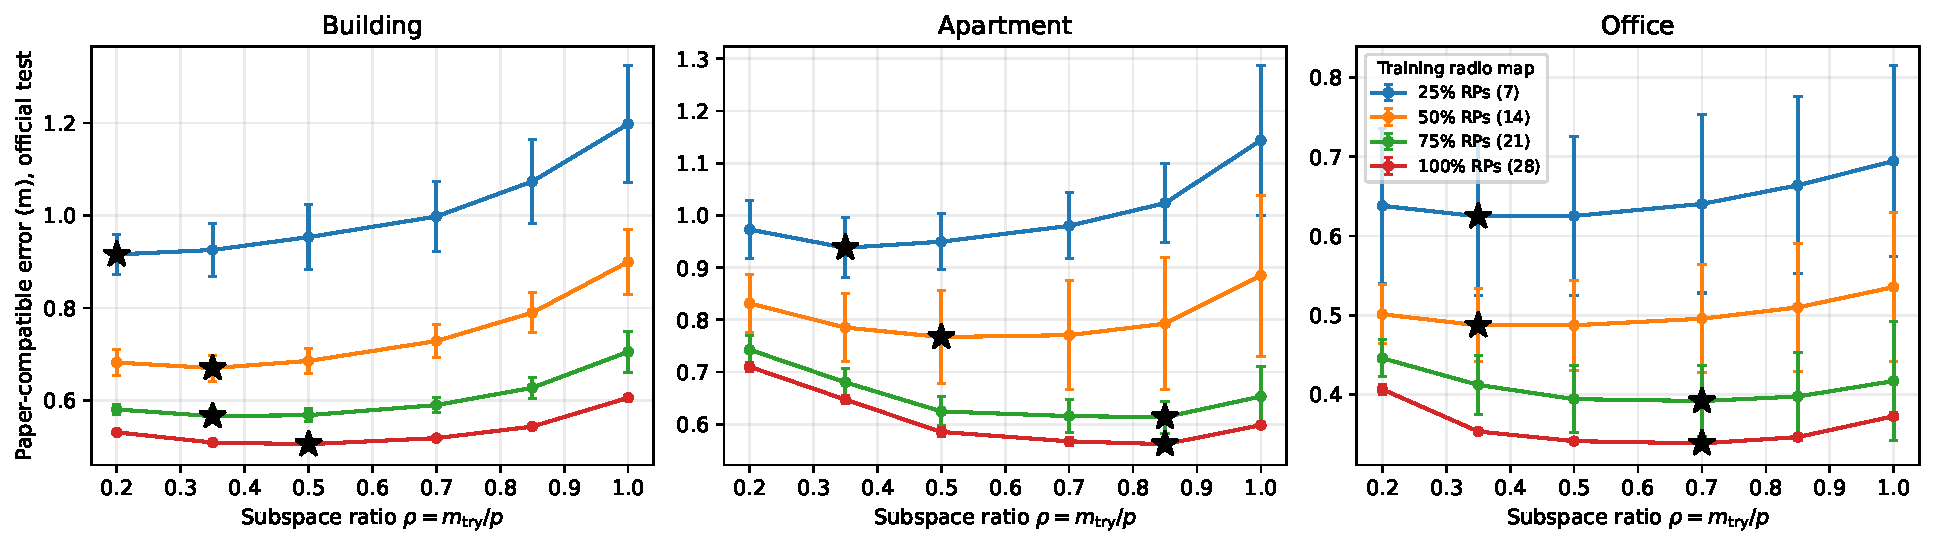
\includegraphics[width=\textwidth]{figures/results/fig13_density_ratio.pdf}
	\caption{Official-test error versus subspace ratio for training radio maps thinned to $100\%$, $75\%$, $50\%$, and $25\%$ of their RPs (number of RPs in parentheses; mean $\pm$ standard deviation over ten random RP subsets). Stars mark the best ratio of each curve.}
	\label{fig:density_ratio}
\end{figure*}

Three observations hold. First, $\rho=1$ is never the best ratio. In Building it is the worst ratio at every density, and in Apartment and Office it is the worst at $50\%$ and $25\%$. Second, the best ratio decreases as the map becomes sparser in all three environments (Table~\ref{tab:density_rf_et}):
\begin{itemize}
	\item Building: from $0.5$ at full density to $0.35$ at $75\%$ and $50\%$, and $0.2$ at $25\%$;
	\item Apartment: from $0.85$ at $100\%$ and $75\%$ (where $0.7$ is within $0.005$~m) to $0.5$ at $50\%$ and $0.35$ at $25\%$;
	\item Office: from $0.7$ at $100\%$ and $75\%$ to $0.35$ at $50\%$ and $25\%$.
\end{itemize}
Third, the gain of the best ratio over bagging tends to increase with sparsity. It rises from $16.6\%$ (full) to $25.5\%$ ($50\%$) in Building and from $6.1\%$ to $18.0\%$ ($25\%$) in Apartment. In Office, with only 28 training RPs (7 at $25\%$), it stays between $6\%$ and $10\%$. The fixed default $\rho=0.7$ improves on $\rho=1$ at every density ($5.2$--$19.0\%$), but on the sparsest maps it leaves part of the attainable gain unused (e.g., $0.998$ versus $0.916$~m in Building at $25\%$).

These results are consistent with per-split randomization acting as regularization~\cite{mentch2020randomization}: predicting positions between sparsely surveyed RPs is a noisier interpolation problem, for which stronger randomization is preferable. To test whether the effect is specific to Random Forests, the same thinned maps were used to train extremely randomized trees~\cite{geurts2006extremely} with the same ratio grid (Table~\ref{tab:density_rf_et}).

\begin{table*}[!t]
\centering
\caption{Density dependence of the optimal subspace ratio for Random Forests and extremely randomized trees (official test, paper-compatible metric, mean over 10 random RP subsets; both models use the same thinned radio maps). Best $\rho$: ratio with the lowest mean error in $\{0.2,0.35,0.5,0.7,0.85,1.0\}$. Gain: reduction of the best ratio relative to $\rho=1$.}
\label{tab:density_rf_et}
\footnotesize
\setlength{\tabcolsep}{4pt}
\begin{tabular}{llcccccc}
\toprule
 & & \multicolumn{3}{c}{Random Forest} & \multicolumn{3}{c}{Extremely randomized trees} \\
\cmidrule(lr){3-5}\cmidrule(lr){6-8}
Dataset & Training map & Best $\rho$ & Error (m) & Gain (\%) & Best $\rho$ & Error (m) & Gain (\%) \\
\midrule
Building & 100\% (483) & 0.50 & 0.505 & 16.6 & 1.00 & 0.545 & 0.0 \\
 & 75\% (362) & 0.35 & 0.566 & 19.8 & 1.00 & 0.594 & 0.0 \\
 & 50\% (242) & 0.35 & 0.670 & 25.5 & 1.00 & 0.696 & 0.0 \\
 & 25\% (121) & 0.20 & 0.916 & 23.6 & 0.50 & 0.971 & 0.4 \\
\midrule
Apartment & 100\% (81) & 0.85 & 0.562 & 6.1 & 1.00 & 0.617 & 0.0 \\
 & 75\% (61) & 0.85 & 0.613 & 6.1 & 1.00 & 0.659 & 0.0 \\
 & 50\% (40) & 0.50 & 0.767 & 13.3 & 1.00 & 0.757 & 0.0 \\
 & 25\% (20) & 0.35 & 0.938 & 18.0 & 1.00 & 0.903 & 0.0 \\
\midrule
Office & 100\% (28) & 0.70 & 0.338 & 9.2 & 1.00 & 0.349 & 0.0 \\
 & 75\% (21) & 0.70 & 0.392 & 6.1 & 1.00 & 0.392 & 0.0 \\
 & 50\% (14) & 0.35 & 0.487 & 9.0 & 0.50 & 0.443 & 0.8 \\
 & 25\% (7) & 0.35 & 0.625 & 10.1 & 1.00 & 0.583 & 0.0 \\
\bottomrule
\end{tabular}
\end{table*}


For extremely randomized trees, the best ratio is $\rho=1$ at almost every density, and feature subsampling never improves the error by more than $0.8\%$. The density dependence is therefore specific to Random Forests. This is consistent with the regularization interpretation: extremely randomized trees already draw their split thresholds at random, which provides strong randomization, so additional feature subsampling has nothing left to regularize. The comparison also shows that the two ensembles are complementary rather than interchangeable: with the best ratio, RF is more accurate in Building at every density, whereas extremely randomized trees are more accurate on the $50\%$ and $25\%$ Apartment and Office maps.

% ============================================================
\subsection{Choosing the Subspace Ratio}
\label{subsec:selection_results}

If the best ratio depends on density, it matters which data are used to choose it. Table~\ref{tab:ratio_selection} reports the test regret of each selection rule; the corresponding error curves are shown in Fig.~S8 of the supplementary material.

\begin{table*}[!t]
\centering
\caption{Selecting the subspace ratio. For each rule, the selected $\rho$ and the resulting regret on the official RP-disjoint test set (percentage above the best ratio of the sweep, $\rho\in\{0.2,0.35,0.5,0.7,0.85,1.0\}$, paper-compatible metric, seed 0). The test set is used only to score the rules, never to select $\rho$.}
\label{tab:ratio_selection}
\footnotesize
\setlength{\tabcolsep}{4pt}
\begin{tabular}{lccccccc}
\toprule
 & \multicolumn{2}{c}{Building} & \multicolumn{2}{c}{Apartment} & \multicolumn{2}{c}{Office} & \\
\cmidrule(lr){2-3}\cmidrule(lr){4-5}\cmidrule(lr){6-7}
Selection rule & $\rho$ & Regret (\%) & $\rho$ & Regret (\%) & $\rho$ & Regret (\%) & Worst (\%) \\
\midrule
Out-of-bag error (sample level) & 0.35 & 1.0 & 0.50 & 1.9 & 0.35 & 6.0 & 6.0 \\
5-fold sample-level CV & 0.35 & 1.0 & 0.50 & 1.9 & 0.35 & 6.0 & 6.0 \\
5-fold RP-grouped CV & 0.35 & 1.0 & 0.50 & 1.9 & 0.20 & 22.5 & 22.5 \\
Leave-one-environment-out minimax (RP-grouped CV) & 0.35 & 1.0 & 0.35 & 12.5 & 0.35 & 6.0 & 12.5 \\
Fixed $\rho=1.0$ (bagging; Feng et al.) & 1.00 & 19.7 & 1.00 & 6.4 & 1.00 & 12.1 & 19.7 \\
Fixed $\rho=0.7$ (this work) & 0.70 & 4.1 & 0.70 & 0.0 & 0.70 & 0.6 & 4.1 \\
Fixed $\rho=0.5$ & 0.50 & 0.0 & 0.50 & 1.9 & 0.50 & 0.0 & 1.9 \\
Fixed $\rho=0.35\approx1/3$ (Breiman) & 0.35 & 1.0 & 0.35 & 12.5 & 0.35 & 6.0 & 12.5 \\
\bottomrule
\end{tabular}
\end{table*}


The OOB error is between $0.04$ and $0.25$~m, an order of magnitude below the test error, because every scan is predicted by trees trained on other scans of the same RP; sample-level CV behaves the same way. Both estimators, and RP-grouped CV, select ratios of $0.2$--$0.5$, smaller than the test optimum ($0.5$--$0.7$). For RP-grouped CV this is the density effect of Section~\ref{subsec:density_results}: its fold models see a sparser map. As a result, the data-driven rules incur worst-case test regrets of $6.0$--$22.5\%$ (the leave-one-environment-out rule $12.5\%$) and bagging $19.7\%$, whereas the fixed default $\rho=0.7$ stays within $4.1\%$ of the best ratio in every environment and $\rho=0.5$ within $1.9\%$. The test curves are flat between $0.5$ and $0.7$, so for fully surveyed maps any ratio in this range is a robust default, while sparser maps favor smaller ratios.

The EETAC sweep (three seeds) is consistent with this picture. EETAC has only 25 RPs, i.e., a sparse map by the standards of Fig.~\ref{fig:density_ratio}, and its within-day sample-level and RP-grouped protocols are best at $\rho=0.35$--$0.5$. Across days, very small ratios become harmful in the seven-AP scenario (2D RMSE $3.19$~m at $\rho=0.2$ for Day~1$\rightarrow$Day~2), presumably because trees are then forced to split on Linksys APs whose measurements change between days, and the best cross-day ratios are $0.5$--$0.85$. In every EETAC protocol and scenario, $\rho=0.7$ is better than $\rho=1$.

% ============================================================
\subsection{Comparison with Literature Ensembles}
\label{subsec:literature_results}

The previous analyses vary only the subspace ratio of one RF. Table~\ref{tab:literature_baselines} places the configuration among other ensembles and a classical fingerprinting baseline: Breiman's default $m_{\mathrm{try}}=\lfloor p/3\rfloor$, extremely randomized trees, Rotation Forest, gradient-boosted trees, and WKNN.

\begin{table*}[!t]
\centering
\caption{Comparison with tree-ensemble and fingerprinting alternatives from the literature (paper-compatible metric, m). Test: official RP-disjoint test set. CV: pooled 5-fold RP-grouped CV on the training RPs. Office and Apartment: mean of three seeds; Building: one seed. Best value per column in bold.}
\label{tab:literature_baselines}
\footnotesize
\setlength{\tabcolsep}{4pt}
\begin{tabular}{lcccccc}
\toprule
 & \multicolumn{2}{c}{Building} & \multicolumn{2}{c}{Apartment} & \multicolumn{2}{c}{Office} \\
\cmidrule(lr){2-3}\cmidrule(lr){4-5}\cmidrule(lr){6-7}
Model & Test & CV & Test & CV & Test & CV \\
\midrule
RF, $\rho=1.0$ (bagging) \cite{feng2026robust} & 0.605 & 0.887 & 0.598 & 0.705 & 0.373 & 0.602 \\
RF, $\rho=0.7$ (this work) & 0.526 & 0.707 & \textbf{0.564} & 0.617 & \textbf{0.339} & 0.464 \\
RF, $m_{\mathrm{try}}=\lfloor p/3\rfloor$ \cite{breiman2001random} & \textbf{0.515} & \textbf{0.649} & 0.640 & 0.621 & 0.351 & 0.424 \\
Extremely randomized trees \cite{geurts2006extremely} & 0.543 & 0.698 & 0.616 & \textbf{0.611} & 0.346 & \textbf{0.386} \\
Rotation Forest \cite{rodriguez2006rotation} & 0.520 & 0.652 & 0.704 & 0.619 & 0.386 & 0.394 \\
Gradient-boosted trees (500 iterations) & 0.620 & 0.765 & 0.834 & 0.683 & 0.352 & 0.431 \\
WKNN, $k=5$ \cite{bahl2000radar} & 0.941 & 1.139 & 0.853 & 0.842 & 0.401 & 0.465 \\
\bottomrule
\end{tabular}
\end{table*}


No method is best everywhere. On the official test sets, RF300-F0.7 is best in Office and Apartment and within $0.011$~m of the best model (RF with $\lfloor p/3\rfloor$) in Building. Under RP-grouped CV, i.e., on sparser maps, the more strongly randomized ensembles lead: extremely randomized trees in Office and Apartment, and RF with $\lfloor p/3\rfloor$ and Rotation Forest in Building. This ordering again matches the density effect. Gradient-boosted trees, a strong general-purpose tabular baseline, are less accurate than RF300-F0.7 on every official test set (e.g., $0.620$ versus $0.526$~m in Building and $0.834$ versus $0.564$~m in Apartment). WKNN, the classical fingerprinting baseline, is clearly worse in the two larger environments. All bagging-based randomized ensembles improve on the full-feature RF used in prior work.

% ============================================================
\subsection{Accuracy--Efficiency Trade-off}
\label{subsec:efficiency_results}

Accuracy is only one side of the comparison. The measured cost of the two 300-tree models is reported in the supplementary material (Table~S7). Wall-clock training and inference times vary with the environment and system load; for example, Building training took $13.63$~s for RF300-F1.0 and $6.35$~s for RF300-F0.7 in this run, with inference times of $12.93$ and $9.29~\mu$s per scan. At equal tree count, the subsampled model is $9$--$19\%$ larger in serialized size, because its trees are deeper.

Fig.~\ref{fig:model_size} (values in Table~S11 of the supplementary material) shows that the accuracy gained by subsampling can be traded for model size. A 100-tree RF0.7 forest matches or slightly improves on the 300-tree RF0.7 forest in all three environments; a 50-tree forest loses $0.004$--$0.010$~m. In Building, the 50-tree RF0.7 forest is $10.7$~MB instead of $58.8$~MB for the 300-tree full-feature model ($5.5\times$ smaller), infers in about $2~\mu$s per scan on one thread instead of about $13~\mu$s, and is still $11.4\%$ more accurate ($0.536$ versus $0.605$~m). The corresponding Office and Apartment models occupy $0.56$ and $2.49$~MB. The compact Building model remains larger than the 93,934-parameter GTCN~\cite{rana2025gtcn}, which reports a lower 2D RMSE ($0.660$~m) at the cost of roughly 38~min of training.

\begin{figure*}[!t]
	\centering
	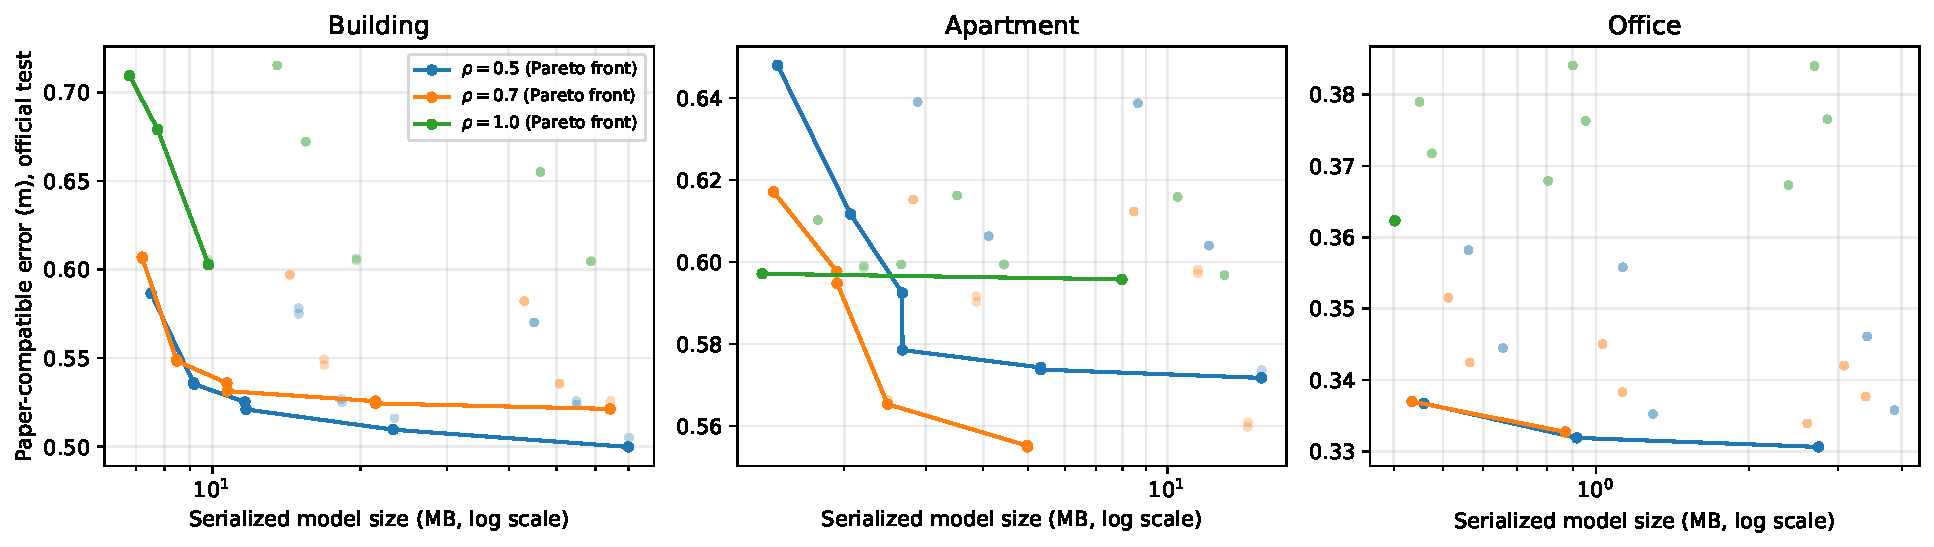
\includegraphics[width=\textwidth]{figures/results/fig15_model_size.pdf}
	\caption{Official-test error versus serialized model size for forests with 50--300 trees, minimum leaf sizes 1--20, and depth limits, for $\rho\in\{0.5,0.7,1.0\}$. Lines show the Pareto front of each ratio.}
	\label{fig:model_size}
\end{figure*}

% ============================================================
\subsection{Uncertainty-Region Performance}
\label{subsec:uncertainty_results}

We finally turn from point accuracy to uncertainty regions. Table~\ref{tab:calibration_rules} compares the three calibration rules of Section~\ref{subsec:strict_conformal} over repeated random RP-level fit/calibration splits. Since the guarantee of split conformal prediction concerns the coverage averaged over calibration draws, the mean coverage is the relevant criterion for validity; the minimum shows how much a single deployment can deviate from it. Reserving calibration RPs has a cost for the point predictor: trained on the $\sim$75\% fitting subset instead of all training RPs, RF300-F0.7 is $13.6\%$ less accurate in Building and $11.7\%$ in Apartment, and essentially unchanged in Office (Table~S10 of the supplementary material).

\begin{table*}[!t]
\centering
\caption{Split-conformal calibration of circular regions when the $\sim$120 scans of each RP are correlated, over repeated random RP-level fit/calibration splits ($25\%$ of training RPs for calibration; coverage on the official test set). Scan-level: all calibration scans treated as exchangeable. Group: one randomly chosen scan per calibration RP, with ordinary split conformal on these $G$ scores, which is valid when RPs are exchangeable~\cite{Dunn02102023}. RP-count: pooled scores with the finite-sample level computed from $G$. The guarantee of a valid method concerns the mean coverage over calibration draws; individual splits vary around it.}
\label{tab:calibration_rules}
\footnotesize
\setlength{\tabcolsep}{4pt}
\begin{tabular}{llcccccc}
\toprule
 & & \multicolumn{3}{c}{$1-\alpha=0.90$} & \multicolumn{3}{c}{$1-\alpha=0.95$} \\
\cmidrule(lr){3-5}\cmidrule(lr){6-8}
Dataset & Calibration rule & Mean cov. & Min cov. & Area (m$^2$) & Mean cov. & Min cov. & Area (m$^2$) \\
\midrule
Building ($G=121$, 10 splits) & Scan-level (standard) & 0.940 & 0.917 & 5.98 & 0.974 & 0.962 & 9.80 \\
 & Group, one scan per RP (valid) & 0.946 & 0.913 & 6.55 & 0.978 & 0.959 & 11.45 \\
 & RP-count (conservative heuristic) & 0.946 & 0.924 & 6.31 & 0.978 & 0.965 & 10.97 \\
\midrule
Apartment ($G=21$, 20 splits) & Scan-level (standard) & 0.894 & 0.838 & 6.63 & 0.931 & 0.895 & 9.12 \\
 & Group, one scan per RP (valid) & 0.916 & 0.871 & 8.10 & 0.947 & 0.897 & 11.88 \\
 & RP-count (conservative heuristic) & 0.932 & 0.896 & 9.25 & 0.995 & 0.968 & 33.19 \\
\midrule
Office ($G=7$, 20 splits) & Scan-level (standard) & 0.947 & 0.809 & 4.09 & 0.958 & 0.853 & 5.02 \\
 & Group, one scan per RP (valid) & \multicolumn{3}{c}{no finite region ($G<1/\alpha-1$)} & \multicolumn{3}{c}{no finite region ($G<1/\alpha-1$)} \\
 & RP-count (conservative heuristic) & 0.980 & 0.898 & 8.88 & 0.980 & 0.898 & 8.88 \\
\bottomrule
\end{tabular}
\end{table*}


With 121 calibration RPs (Building), the three rules agree: all over-cover moderately ($0.94$--$0.98$), and the group and RP-count regions are $5$--$17\%$ larger than the scan-level ones. With $G=21$ (Apartment), the scan-level rule falls below the nominal level on average ($0.894$ at $90\%$, $0.931$ at $95\%$) and under-covers in $65\%$ and $75\%$ of the splits. The group rule, which uses one scan per RP and is valid when RPs are exchangeable~\cite{Dunn02102023}, restores the nominal mean coverage ($0.916$ and $0.947$) with regions $22$--$30\%$ larger. Individual splits still fall below the nominal level, as expected for a marginal guarantee with only 21 calibration scores. The RP-count correction over-covers ($0.932$ and $0.995$); at $95\%$, where $G<2/\alpha-1$, its threshold is the largest pooled score and the region grows to $33.2$~m$^2$, nearly three times the group region.

With $G=7$ (Office), the group rule has no finite region at either level, because $G<1/\alpha-1$. The scan-level rule gives finite regions but under-covers in $25$--$35\%$ of the splits (minimum $0.809$), and the RP-count heuristic has no guarantee. Seven calibration RPs are therefore too few for a valid circle at these levels. In general, a valid group calibration needs at least $1/\alpha-1$ held-out RPs (9 at $90\%$, 19 at $95\%$), and its region shrinks toward the scan-level region as $G$ grows. This gives a direct survey-planning rule for uncertainty-aware fingerprinting.

The single-split results in the supplementary material (Table~S8) compare circles with covariance-aware ellipses. With scan-level calibration, the ellipse is $3.7$--$7.8\%$ smaller than the circle under split conformal and $6.0$--$13.0\%$ smaller under grouped OOF. Its coverage is close to that of the circle in Building but lower in Office and Apartment, so the ellipse is a more compact anisotropic description of the error, not a better-calibrated region.

% ============================================================
\subsection{Summary of Main Findings}
\label{subsec:results_summary}

The main findings of this section are:

\begin{itemize}
	\item Full-feature bagging is never the best ratio; RF300-F0.7 reduces the reproduced baseline error by $14.3\%$, $7.1\%$, and $5.1\%$ on the official tests (significant for Building and Office; lower error in all ten seeds in every environment) and by $20.1\%$, $22.1\%$, and $12.2\%$ under RP-grouped CV.
	\item For Random Forests, the optimal ratio decreases as the radio map becomes sparser in all three environments, and the gain over bagging reaches $25.5\%$; extremely randomized trees gain at most $0.8\%$ from subsampling. The fixed default $\rho=0.7$ is within $4.1\%$ of the best ratio at full density, whereas OOB, sample-level, and RP-grouped selection are biased toward small ratios.
	\item On the frame-aligned EETAC dataset, RF300-F0.7 improves 2D RMSE by $11$--$14\%$ in sample-level and RP-grouped CV and is better in 74 of 80 seed--protocol comparisons; one cross-day direction (High, Day~1$\rightarrow$Day~2) is a tie.
	\item No literature ensemble is best everywhere; the strongest one depends on map density, randomized bagging ensembles all improve on the full-feature RF, and gradient boosting and WKNN are less accurate.
	\item 50--100-tree subsampled forests are more accurate than the 300-tree full-feature forest while being $2.5$--$5.5$ times smaller.
	\item With 21 calibration RPs, scan-level conformal calibration falls below the nominal coverage on average, whereas group calibration with one scan per RP attains it with $22$--$30\%$ larger regions; with 7 RPs no valid finite region exists, and the RP-count heuristic is conservative.
\end{itemize}

\section{Discussion}
\label{sec:discussion}

The results show a consistent improvement of feature subsampling over the full-feature forest used in prior hybrid RTT--RSS work, but also that the size of this improvement, and the best subsampling ratio, depend on the evaluation protocol through one common factor: the density of the training radio map. This section interprets these findings and their implications for fingerprinting practice.

% ============================================================
\subsection{Why Feature Subsampling Helps, and Why It Helps More on Sparse Maps}
\label{subsec:discussion_subspace}

RF300-F0.7 differs from RF300-F1.0 only in the number of candidate features per split. With $\rho=1$, the forest is bagging: every tree sees the same features at every split and differs only through its bootstrap sample. Hybrid fingerprints are a favorable setting for decorrelation, because the RTT and RSS of one AP and the measurements of neighboring APs carry overlapping position information, and because the usefulness of an AP changes across space with LOS/NLOS conditions and visibility. Without subsampling, the same few dominant features drive most splits of most trees, so the trees make correlated errors at locations where those features are unreliable.

The density experiment adds a second, more specific explanation. Per-split randomization reduces the effective degrees of freedom of a forest and is most useful when the signal-to-noise ratio is low~\cite{mentch2020randomization}. In fingerprinting, the test scans lie between surveyed RPs; the sparser the radio map, the farther the nearest training RP and the noisier the interpolation problem. Consistently, the best ratio decreases in all three environments as RPs are removed from the training map, and the gain over bagging tends to increase (Fig.~\ref{fig:density_ratio}), and the more strongly randomized literature ensembles lead under grouped CV but not on the full-density test (Table~\ref{tab:literature_baselines}). The same mechanism explains why the relative gain of RF300-F0.7 is larger under RP-grouped CV than on the official test. It also explains a boundary of the effect: extremely randomized trees, which already draw random split thresholds, are strongly regularized without feature subsampling and gain at most $0.8\%$ from it at any density (Table~\ref{tab:density_rf_et}). The density dependence is therefore a property of Random Forests, whose only sources of randomness are the bootstrap and the feature subset.

Differences between environments fit the same picture. The Building environment benefits most at full density. It has the most APs ($p=26$), mixed LOS/NLOS conditions, and the largest area, which provides more redundant and locally unreliable features for subsampling to decorrelate. Office ($p=6$) and Apartment ($p=8$) offer few features, so a ratio of $0.7$ removes only two or three candidates per split.

% ============================================================
\subsection{Choosing the Ratio: A Fixed Default Beats Validation-Based Selection}
\label{subsec:discussion_selection}

A practitioner would normally tune $m_{\mathrm{try}}$ with out-of-bag error or cross-validation~\cite{probst2019hyperparameters}. In fingerprinting, both shortcuts are misleading. OOB and sample-level CV errors are an order of magnitude below the test error because each scan is evaluated by trees that have seen other scans of the same RP; they measure recognition, not localization. RP-grouped CV is unbiased with respect to leakage but evaluates models trained on a sparser map than the deployed model, and the density effect then pushes it toward ratios that are too small; in Office, it selects $\rho=0.2$ and incurs a $22.5\%$ test regret. A fixed default in the flat region of the full-density curves, $0.5$--$0.7$, is more reliable: $\rho=0.7$ has a worst-case regret of $4.1\%$ against $19.7\%$ for bagging.

Two practical rules follow. For a fully surveyed radio map, a ratio between $0.5$ and $0.7$ is a safe default. For a sparse map, or when RPs are reserved for validation or calibration, a smaller ratio around $0.35$ is preferable. A validation-based choice should account for the density difference between validation and deployment models, for instance by tuning at matched density.

We emphasize that $\rho=0.7$ was not selected by these analyses: it was fixed during development and frozen before the external evaluation, and the analyses quantify how far it is from the best ratio in hindsight. Choosing $0.5$ now, because it has a slightly lower regret on these test sets, would amount to tuning on the test data.

% ============================================================
\subsection{External and Cross-Day Validation}
\label{subsec:discussion_external}

A fixed default is only useful if it transfers. The EETAC experiments are external in three respects: a different building, smartphone, and AP deployment. After frame alignment, RF300-F0.7 reduces the sample-level and RP-grouped 2D RMSE by 11--14\%, with bootstrap intervals that exclude zero, and is better in 74 of 80 seed--protocol comparisons. EETAC's 25-RP grid is a sparse radio map, and its within-day protocols indeed prefer ratios of $0.35$--$0.5$, which again matches the density effect, while $\rho=0.7$ still improves on $\rho=1$ everywhere.

The cross-day results change substantially once the acquisition-day frames are aligned: errors drop from more than $5$~m to $1.2$--$1.7$~m. Temporal shift remains real, since cross-day errors are about four times the within-day sample-level errors, but it is far smaller than the misaligned data suggest. Under this shift, RF300-F0.7 gives its largest relative gains ($13$--$20\%$ for Day~2$\rightarrow$Day~1 over ten seeds), which is consistent with decorrelated trees being less dependent on individual APs whose measurements drift between days. The effect is not uniform, however: in the seven-AP scenario, Day~1$\rightarrow$Day~2 is a tie. The seven-AP sweep also shows the limit of this argument: at $\rho=0.2$, trees are forced to rely on unstable Linksys APs, and cross-day error rises to $3.2$~m.

The frame mismatch is itself a methodological lesson. Pooled or cross-day experiments implicitly assume that coordinates mean the same thing in every file. A simple fingerprint-consistency check, such as matching per-RP median RTT fingerprints across acquisition days, is cheap and detects such errors before they are interpreted as radio-map drift.

% ============================================================
\subsection{Mean Accuracy and Tail Robustness}
\label{subsec:discussion_tail}

The average improvements discussed above do not tell the whole story, because an improvement in RMSE does not guarantee an improvement throughout the error distribution. In the Apartment official test, RF300-F0.7 lowers the RMSE in all ten seeds but raises $P_{90}$ in all ten, and the bootstrap interval of the single-seed improvement includes zero. On EETAC under sample-level CV, the full-feature forest returns the exact grid coordinates for most scans of already-surveyed RPs, which gives it a lower $P_{90}$; RF300-F0.7 trades this exact recognition for fewer large errors, which lowers the RMSE. Applications that only need to identify a surveyed RP and those that need continuous positions therefore favor different trade-offs. Reporting RMSE, mean error, and several percentiles together, as done here, makes these differences visible.

% ============================================================
\subsection{Environment-Dependent Importance of RTT and RSS}
\label{subsec:discussion_modalities}

The way subsampling helps also depends on the two modalities. The feature importances show that RTT dominates in Building and Apartment, whereas RTT and RSS contribute more evenly in Office. Hybrid positioning should therefore not be seen as a fixed weighting of the two modalities. Subsampling lets different trees rely on different modalities and APs, so the ensemble can represent several complementary RTT--RSS relationships without an explicit weighting rule. In a screening experiment, drawing one feature subset per tree (Ho's random subspace method~\cite{ho1998random}) instead of per split was worse in all three environments (e.g., Apartment test error $0.645$~m versus $0.564$~m), and drawing whole APs, i.e., keeping each AP's RTT and RSS together, did not change this ($0.648$~m). The benefit therefore comes from per-split randomization rather than from a particular grouping of the modalities.

% ============================================================
\subsection{Efficiency and Model Size}
\label{subsec:discussion_efficiency}

At equal tree count, subsampling does not consistently change training or inference time, and it slightly increases model size because the trees grow deeper. The efficiency argument therefore rests on a different observation: the accuracy gained by subsampling can be spent on a smaller forest. A 50--100-tree subsampled forest remains more accurate than the 300-tree full-feature forest while being $2.5$--$5.5$ times smaller, trains in about one second on Building, and infers in a few microseconds per scan on one CPU thread.

This should not be confused with state-of-the-art accuracy. GTCN~\cite{rana2025gtcn} reports a lower 2D RMSE on the Building environment ($0.660$~m versus $0.732$~m) with a much smaller parameter count. Its reported training time, about 38~min for 1500 epochs, compares with 6--15~s for the 300-tree subsampled forest and about 1~s for the 50-tree forest on our laptop CPU, i.e., two to three orders of magnitude less. Because the two timings come from different hardware and implementations, this ratio indicates an order of magnitude rather than a precise speed-up. The subsampled forest therefore occupies a different point of the design space: no GPU, no iterative training or learning-rate schedule, retraining in seconds after a radio-map update, and an accuracy about $11\%$ below that of the graph--temporal network. Which point is preferable depends on how often the model must be retrained and on the hardware available for training.

% ============================================================
\subsection{Relationship to Recent Low-Complexity RTT Localization}
\label{subsec:discussion_recent_methods}

Gonzalez Diaz et al.~\cite{gonzalezdiaz2026scalable} optimize RTT positioning for IoT scalability by limiting which APs are ranged and by lightweight proximity-based processing. The present work addresses a complementary question: how a hybrid RTT--RSS regressor should be configured and evaluated once the measurements are available. Because the two studies differ in datasets, AP subsets, error definitions, and protocols, we do not compare their numbers directly; the EETAC experiments here demonstrate transferability of the RF configuration rather than superiority over that framework.

% ============================================================
\subsection{Uncertainty Regions and Calibration with Clustered Scans}
\label{subsec:discussion_uncertainty}

The covariance-aware ellipse is consistently smaller than the circle because it adapts to the anisotropy of the residuals, which in indoor environments follows corridor orientation, AP geometry, and walls. Its coverage, however, is not better than that of the circle, so its benefit is a more compact description of the error rather than improved calibration.

The more consequential finding concerns calibration itself. The finite-sample guarantee of split conformal prediction holds for exchangeable calibration and test units. In a fingerprinting dataset, the units are RPs, each represented by $\sim$120 nearly identical scans. Treating scans as independent inflates the apparent calibration sample size by two orders of magnitude, so the scan-level threshold is effectively an estimate from $G$ RPs without the corresponding finite-sample margin. With $G=121$ (Building) this is harmless. With $G=21$ (Apartment), the scan-level rule falls below the nominal coverage on average, which is a failure of validity rather than of a single unlucky split. Group calibration with one scan per RP~\cite{Dunn02102023} restores the nominal mean coverage at a moderate cost in area ($22$--$30\%$), whereas the RP-count heuristic is conservative and, when $G<2/\alpha-1$, degenerates to the largest pooled score. With $G=7$ (Office), no valid finite circle exists at the $90\%$ and $95\%$ levels. In practice, the number of calibration RPs, not the number of calibration scans, should be planned: a valid construction needs at least 9 calibration RPs for $90\%$ and 19 for $95\%$, and more RPs shrink the region toward the scan-level one. This requirement conflicts with the cost of withholding RPs from the point predictor, which the density effect explains ($12$--$14\%$ higher error with $75\%$ of the RPs), and motivates cross-fitted methods such as group-aware jackknife+ or CV+~\cite{barber2021jackknife,Dunn02102023}.

The full-training grouped-OOF variant uses all RPs for the point predictor and produces smaller regions with good empirical coverage here, but it does not inherit the split-conformal guarantee because its scores come from several fold models.

% ============================================================
\subsection{Practical Implications}
\label{subsec:discussion_practical}

Taken together, the findings translate into five recommendations for tree-based RTT--RSS fingerprinting:

\begin{enumerate}
	\item Prefer per-split feature subsampling to full-feature forests for hybrid RTT--RSS fingerprinting: it generally improves average localization accuracy at negligible tuning cost, although the benefit is not universal across tail metrics and temporal conditions.
	\item Use a ratio of about $0.5$--$0.7$ for densely surveyed maps and a smaller one for sparse maps; do not tune it with OOB or sample-level CV.
	\item Evaluate on complete held-out RPs and report sample-level results separately; verify coordinate consistency across acquisition sessions before pooling them.
	\item Report mean and tail metrics with RP-clustered confidence intervals, since a few test RPs can dominate the comparison.
	\item Calibrate conformal regions at the RP level, e.g., with one score per calibration RP, and reserve at least $1/\alpha-1$ RPs for the desired confidence level.
\end{enumerate}

% ============================================================
\subsection{Overall Interpretation}
\label{subsec:discussion_overall}

The contribution of this work is not a new learning paradigm. Random feature subsampling is a well-established principle. What this study adds is a characterization of this one design variable for hybrid RTT--RSS fingerprinting: its effect relative to current practice, its dependence on radio-map density, how it should and should not be chosen, how it transfers to an independent dataset and across days, and how it interacts with model size and with calibration. The evidence comes from the consistency of the effect across three benchmark environments, four survey densities, two AP configurations of an external dataset, cross-day transfer, ten seeds, and several literature baselines, and from the identified boundaries: no universal improvement of tail metrics, a non-significant single-seed official-test gain in the smallest test set, a cross-day tie in one direction, environment-dependent best ratios, and calibration that requires enough reference points.

\section{Limitations}
\label{sec:limitations}

\textbf{Environments, devices, and seeds.} The study covers three benchmark environments and one external auditorium, recorded with two smartphone models. It is not a cross-device study, and RTT and RSS are known to depend on chipset, antenna, and firmware. The main tables use one seed; the headline comparison and the EETAC protocols were repeated with ten seeds, but the Building literature-baseline and selection-rule analyses use one seed because of their cost. At full radio-map density, the seed standard deviation of the paper-compatible metric is at most $0.008$~m, well below the differences between $\rho=0.7$ and $\rho=1$ but comparable to some differences among the randomized ensembles of Table~\ref{tab:literature_baselines}. The bootstrap intervals resample test RPs for a fixed model and do not include seed variability.

\textbf{The subspace ratio.} $\rho=0.7$ is a robust default, not the optimum: at full density, the best ratios are $0.5$--$0.85$, and on sparser maps they are smaller. The decrease of the best ratio with density is observed in all three environments, but for Random Forests only, and in Office (28 training RPs) the gain over bagging does not grow with sparsity; extremely randomized trees hardly benefit from feature subsampling at all. A rule that sets $\rho$ from radio-map density, AP count, or modality reliability is suggested by the results but not developed or validated.

\textbf{Development exposure.} The original benchmark was used during method development, so its official-test improvements are not results on a completely untouched benchmark. This is one reason for the external EETAC evaluation, for which $\rho$ was frozen beforehand. In the extension analyses, the official tests score alternatives in hindsight but are never used to choose the proposed configuration. Moreover, the Apartment improvement on the official test is not significant on its own (its bootstrap interval includes zero), although it occurs in all ten seeds.

\textbf{EETAC.} The mirrored frame of the second acquisition day is inferred from the data (22 of 25 RPs match the mirrored positions, and the identity matches only the mirror-invariant central row). The inference is strong but has not been confirmed by the dataset authors, and which day uses the original frame cannot be determined from the files; accuracy does not depend on this choice. The $5\times5$ grid is a sparse radio map, so RP-disjoint EETAC errors (2.4--2.9~m) are not representative of densely surveyed deployments, and the two-AP configuration of~\cite{gonzalezdiaz2026scalable} could not be reproduced unambiguously.

\textbf{Temporal robustness.} Temporal shift is evaluated with a single pair of acquisition days in one environment, and in one of the four cross-day comparisons the two models tie. Longer time spans, changes in occupancy or furniture, and AP replacement are not covered.

\textbf{Tail errors.} The configuration improves average metrics but not every tail statistic: the Apartment official-test $P_{90}$ and the EETAC sample-level $P_{90}$ are worse than for the full-feature forest. Applications with strict worst-case requirements need mechanisms that target the tail.

\textbf{Uncertainty.} The covariance-aware ellipse reduces area but does not improve coverage. The group calibration is valid only if RPs are exchangeable, which a regular survey grid satisfies only approximately; it discards all but one scan per RP and gives no finite region with fewer than $1/\alpha-1$ calibration RPs. The RP-count correction is a conservative heuristic without a finite-sample guarantee, and it degenerates to the largest calibration score when fewer than $2/\alpha-1$ RPs are available. The full-training grouped-OOF variant has no finite-sample guarantee. Locally normalized scores based on the spread of the tree predictions~\cite{lei2018distribution} reduced the area by $25\%$ at equal coverage in Apartment but over-covered in Building in a screening experiment and are left for future work.

\textbf{Efficiency and comparison.} Timing and model size are measured in Python on a laptop CPU; energy, peak memory, and latency on a phone or embedded device are not measured. Deep learning models are not re-implemented, and the comparison with GTCN relies on its published Building result~\cite{rana2025gtcn}, which is more accurate than the forests studied here. Claims are therefore limited to the experimentally verified comparisons.

\textbf{Feature importance.} The modality analysis relies on impurity-based RF importance, which describes the fitted models and can be redistributed among correlated features; it does not measure the intrinsic value of RTT relative to RSS.

\section{Conclusion}
\label{sec:conclusion}

This study examined the number of candidate features per split as a design variable of hybrid Wi-Fi RTT--RSS Random Forest localization, where prior work has used the full-feature setting, i.e., bagging of regression trees. On three public environments, restricting each split to $70\%$ of the RTT--RSS features reduced the error of the reproduced full-feature baseline by $14.3\%$, $7.1\%$, and $5.1\%$ on the official RP-disjoint test sets, with RP-clustered bootstrap intervals that exclude zero for Building and Office and a lower error in all ten seeds in every environment, and by $12$--$22\%$ under RP-grouped cross-validation.

The ratio analysis explains these numbers. Full-feature bagging was never the best ratio. The optimal ratio decreased in all three environments as the training radio map was thinned, and the gain of subsampling reached $25.5\%$, which is consistent with per-split randomization acting as regularization for the harder interpolation problem posed by sparse maps; extremely randomized trees, which are already strongly randomized, gain at most $0.8\%$ from subsampling. The same effect biases RP-grouped cross-validation toward small ratios, while out-of-bag and sample-level validation are dominated by repeated scans of the same RP. The fixed default $\rho=0.7$ stayed within $4.1\%$ of the best ratio in every environment, compared with $19.7\%$ for bagging, and ratios between $0.5$ and $0.7$ are recommended for densely surveyed maps.

The improvement transferred. On the independent EETAC dataset, the frozen configuration was better than the baseline in 74 of 80 seed--protocol comparisons, including three of the four cross-day directions; the fourth is a tie. This evaluation required correcting a mirrored coordinate frame between the two acquisition days. Without the correction, cross-day errors exceed $5$~m; with it, they are $1.2$--$1.7$~m. The accuracy gained by subsampling also allows smaller models: 50--100-tree forests remained more accurate than the 300-tree full-feature forest while being $2.5$--$5.5$ times smaller. Accuracy remains below that of a recent graph-temporal network on the largest environment, at a small fraction of its training cost.

For uncertainty, covariance-aware ellipses describe anisotropic errors more compactly than circles, but the main lesson concerns calibration: because the scans of an RP are near-duplicates, the effective calibration sample size is the number of RPs. With 21 calibration RPs, scan-level split-conformal regions fell below the nominal coverage on average, whereas group calibration with one scan per RP attained it with $22$--$30\%$ larger regions; with 7 RPs, no valid finite region exists. Calibration should therefore be planned in terms of reference points rather than scans, with at least $1/\alpha-1$ calibration RPs.

Future work will develop a density-aware rule for the subspace ratio, cross-fitted group-conformal calibration that does not withhold RPs from the point predictor, longer-term temporal evaluations, additional buildings and devices, and on-device measurements of compact forests.

\section*{Code and Data Availability}

The code, the experiment outputs, and a Jupyter notebook that reproduces every table and figure of this paper are available at \url{https://github.com/nna17/wifi-rtt-rss-feature-subsampling} and archived at \textbf{[Zenodo DOI]} (release \textbf{[tag, e.g., v1.0]}). The repository contains the main experiment pipeline, the extension and screening experiments, the scripts that generate all tables and figures from the experiment outputs, the exact package versions used (Python 3.14, scikit-learn 1.9.1), and step-by-step instructions; with the included outputs, the tables and figures can be regenerated in seconds without rerunning the experiments. The notebook additionally checks that every number reported in this paper matches the experiment outputs.

The hybrid RTT--RSS benchmark of Feng et al.~\cite{feng2026robust} is available at \url{https://doi.org/10.5281/zenodo.11558192} and \url{https://github.com/Fx386483710/WiFi-RTT-RSS-dataset}. The EETAC auditorium dataset~\cite{martinescalona2023ftm} is available at \url{https://github.com/imartin-UPC/RTT-Data-Collection}. The datasets are not redistributed with the code; the repository describes where to place them.

\section*{CRediT Authorship Contribution Statement}

\textbf{Nabil Abdelkader Nouri:} [roles to be confirmed by the authors]. \textbf{Salim Naouri:} [roles to be confirmed by the authors].

\section*{Declaration of Competing Interest}

The authors declare that they have no known competing financial interests or personal relationships that could have appeared to influence the work reported in this paper.

\section*{Declaration of Generative AI and AI-Assisted Technologies in the Writing Process}

During the preparation of this work, the authors used Claude (Anthropic) to assist in reviewing and extending the experiment scripts and in drafting and editing the manuscript text. After using this tool, the authors reviewed and edited the content as needed and take full responsibility for the content of the published article.

\section*{Acknowledgements}

The authors thank X.~Feng, K.~A.~Nguyen, and Z.~Luo, and E.~Zola and I.~Mart\'in-Escalona, for making their datasets publicly available. [Funding statement, or: This research did not receive any specific grant from funding agencies in the public, commercial, or not-for-profit sectors.]


\bibliographystyle{elsarticle-num}
\bibliography{references_recent_wifi_rtt_rss}

\end{document}
